\documentclass[12pt, a4paper]{article}

\usepackage[utf8]{inputenc}
\usepackage{geometry}
\geometry{top=1in, bottom=1in, left=1in, right=1in}
\usepackage{hyperref}
\usepackage{graphicx}
\usepackage{titling}
\usepackage{float}
\usepackage{booktabs}
\usepackage{array}
\usepackage{caption}

\title{\textbf{Final Report: System Dynamics Modeling of the Effect of Greenhouse Gases on Himalayan Ice Cover in Nepal}}
\author{
    Anishek Kumar Chaudhary (24M0787) \and
    Pratik Man Shah (24M0856) \and
    Ritika Jaiswal (24M0855) \and
    Rohit Agrawal (24M0744)
}
\date{}

\begin{document}

\maketitle

% ============================================================
\section{Summary}
% ============================================================

Nepal's Himalayan glaciers are retreating at an accelerating pace, driven by rising greenhouse gas concentrations, reduced surface albedo, and the deposition of black carbon from South Asian combustion sources. This report presents a system dynamics model that simulates the coupled dynamics of atmospheric carbon accumulation, glacial mass balance, glacial lake expansion, forest cover, and black carbon from 1980 to 2080.

The model captures four reinforcing feedback loops that together push the system toward accelerating glacier loss. The first loop (R1) links ice retreat to lower surface albedo, which absorbs more solar radiation and raises temperatures further. The second (R2) describes how glacial lake growth drives thermal undercutting at glacier termini, feeding melt back into the lake. The third (R3) represents the permafrost carbon trap, where warming beyond a threshold unlocks stored carbon dioxide from frozen soils. The fourth (R4) links black carbon deposition directly to enhanced melt through albedo darkening and direct solar absorption. Two balancing loops moderate the system: the ocean carbon sink (B1) and the terrestrial sink through forest cover (B2), though the terrestrial sink operates at a scale too small relative to global emissions to provide meaningful stabilization.

Under business as usual conditions, the model projects glacier volume falling from 312 km\textsuperscript{3} in 1980 to approximately 155 km\textsuperscript{3} by 2080, a loss of roughly 50 percent. The most effective single policy we tested was black carbon emission reduction, which reduced the GLOF risk index from 0.68 to 0.57 by 2080 and preserved additional glacier volume through the albedo pathway. Combining this with a slowdown in human emission growth delivered the most well rounded outcome across all tracked variables.

% ============================================================
\section{Problem Definition and Reference Mode}
% ============================================================

\subsection{The Problem}

Nepal hosts 3,808 glaciers covering approximately 3,902 km\textsuperscript{2}, storing an estimated 312 km\textsuperscript{3} of ice that supplies freshwater to millions of people across the Hindu Kush Himalayan region \cite{icimod2023}. Sustained greenhouse gas accumulation in the atmosphere is raising global mean temperatures, and the Himalayan cryosphere is particularly sensitive to this warming. The system we model spans the following components: global atmospheric carbon stock, surface temperature at glacial altitudes in Nepal, glacier and snow mass balance, proglacial lake dynamics and glacial lake outburst flood (GLOF) risk, forest cover and its carbon sequestration function, and atmospheric black carbon deposition.

The system boundary is deliberately regional. Human emissions are treated as an exogenous global driver rather than as something Nepal can control locally. The primary concern is how that global forcing propagates through local physical feedbacks to determine how much glacier ice Nepal retains over the next century, and how the risk of GLOF events evolves as a consequence.

\subsection{Reference Mode}

Figure \ref{fig:refmode} shows the reference mode behavior of glaciers volume under the base case scenario from the model. The trajectory shows a slow initial decline through the 1980s and 1990s, followed by a steadily steeper downward curve after 2000 as warming accumulates. This S shaped depletion pattern is consistent with observed satellite data from Brun et al. \cite{brun2017} and the ICIMOD HI-WISE report \cite{icimod2023}, which document accelerating mass loss across High Mountain Asia since 2000.

\begin{figure}[H]
    \centering
    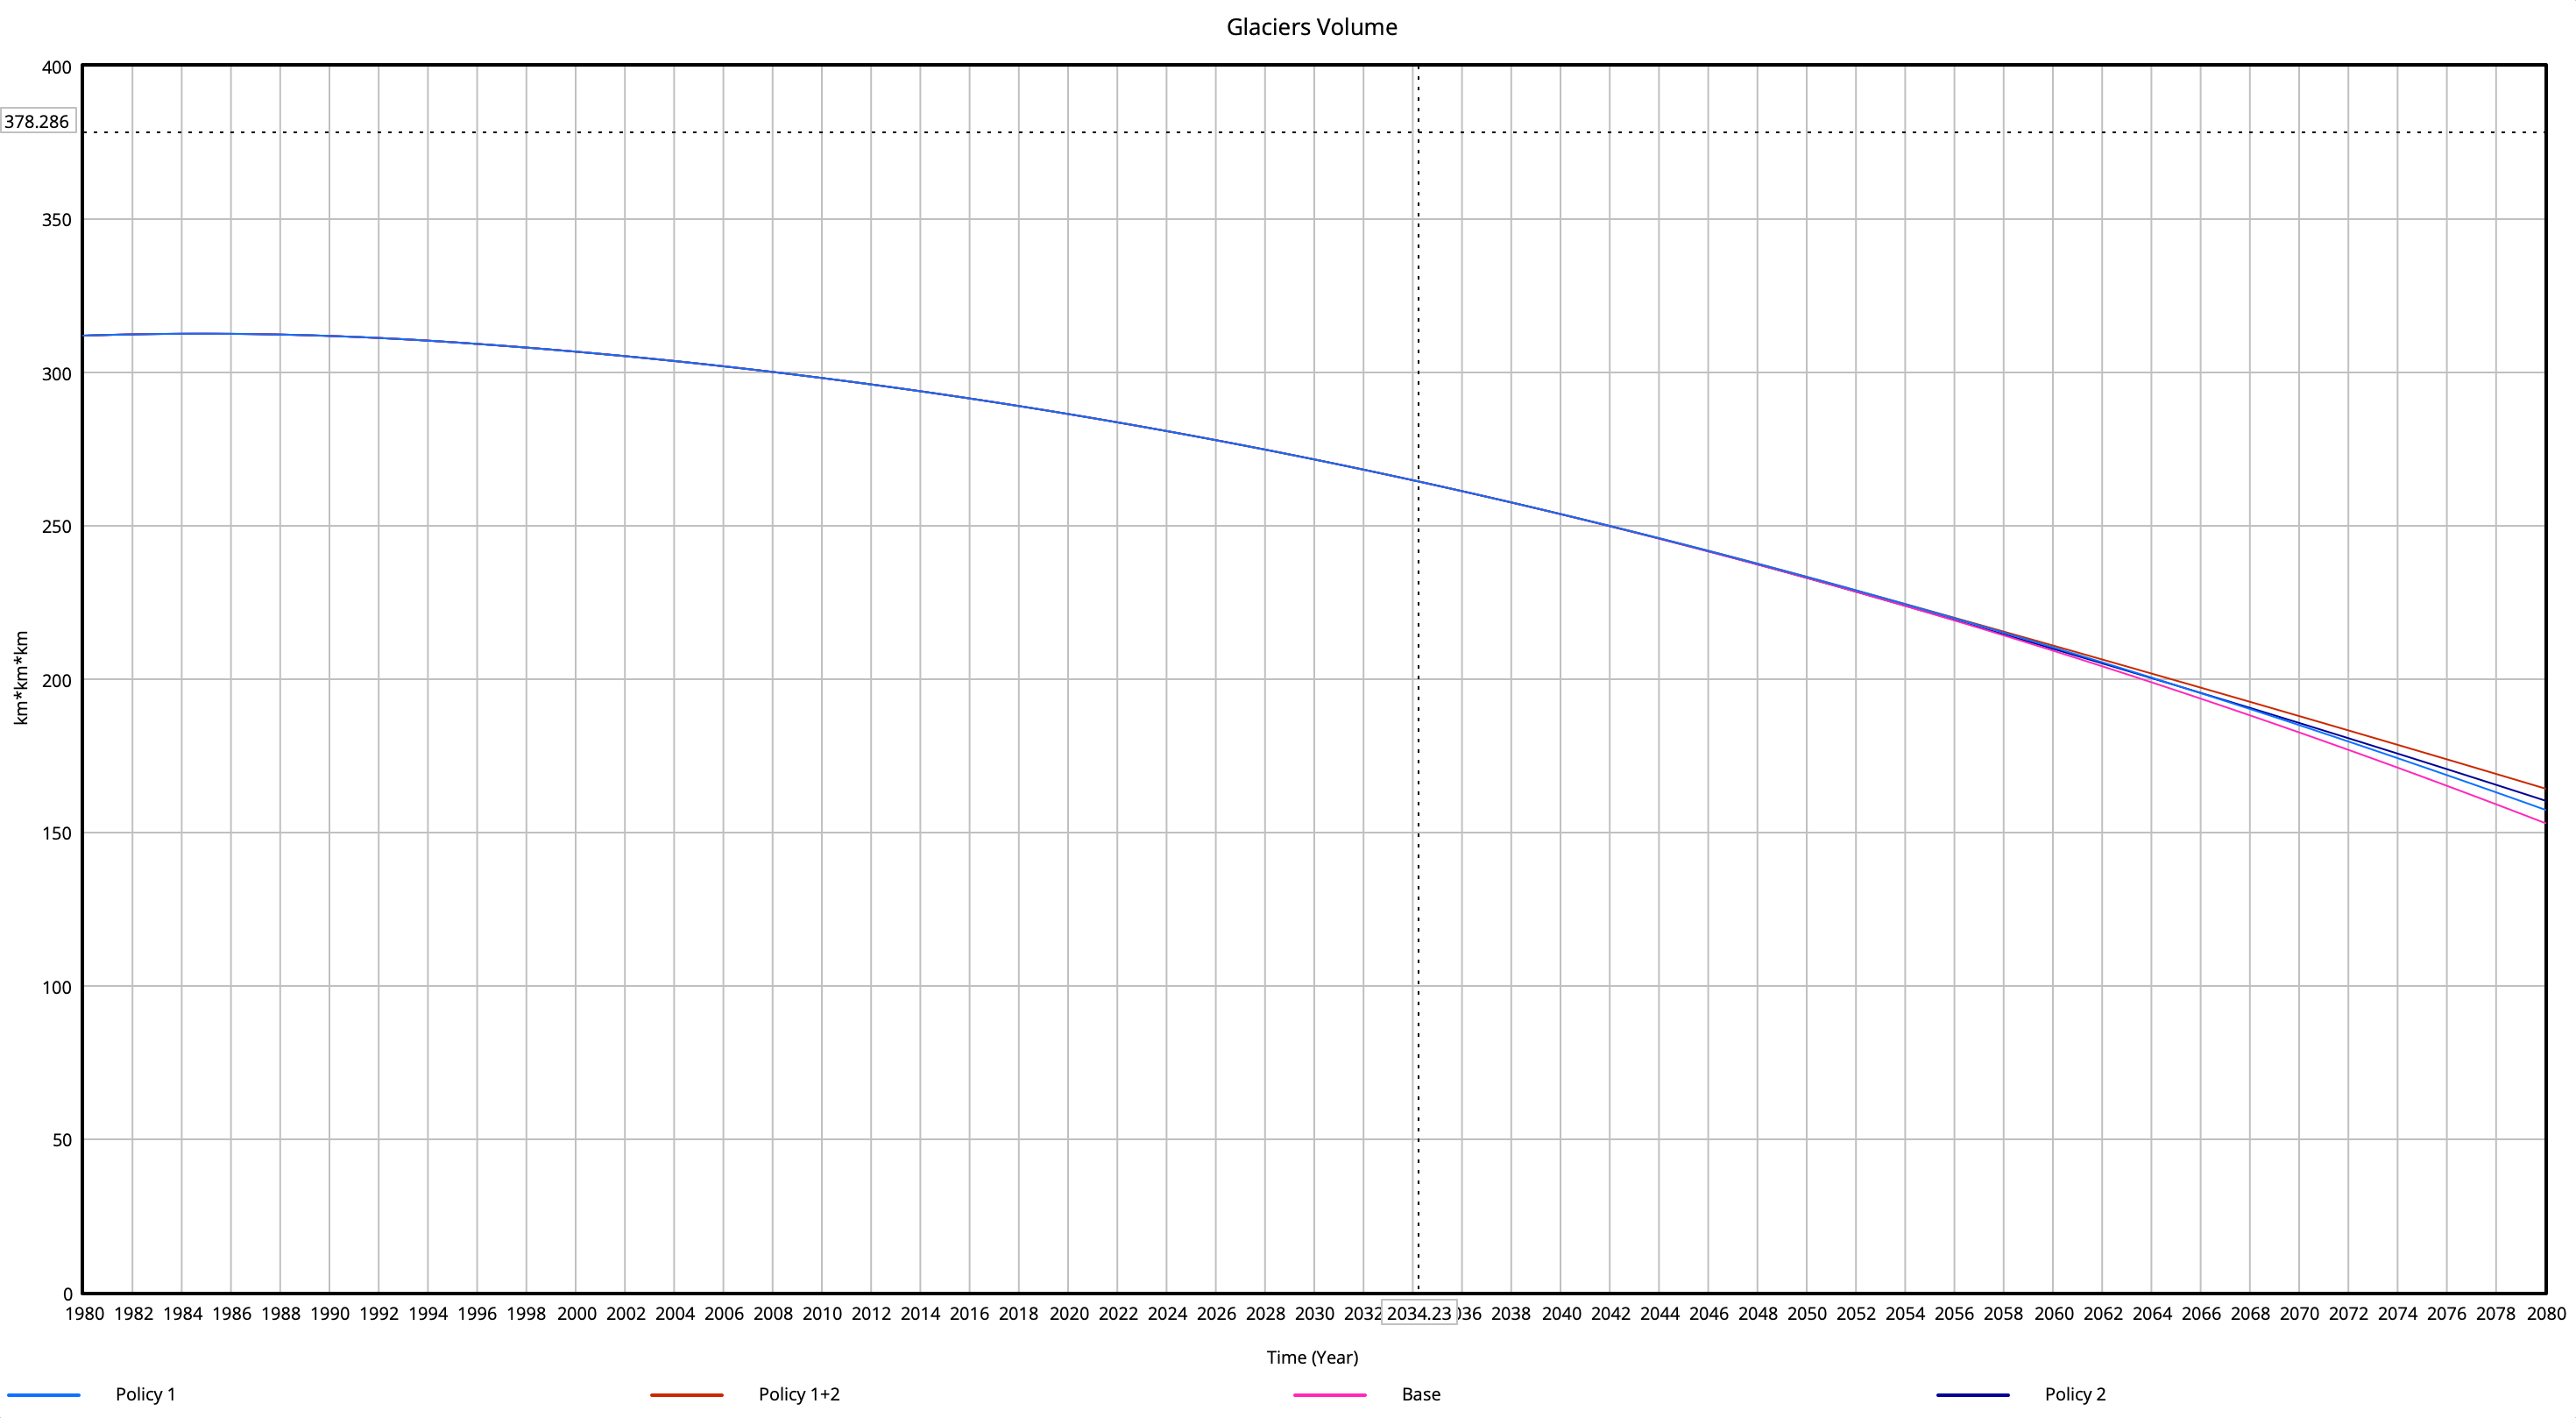
\includegraphics[width=0.9\textwidth]{Updated_Graphs/Graphs_for_policy_1&2/Glaciers Volume.png}
    \caption{Reference mode: Glaciers Volume declining from 312 km\textsuperscript{3} in 1980 to approximately 155 km\textsuperscript{3} by 2080 under base case conditions. The base case (pink line) shows the characteristic accelerating loss pattern driven by reinforcing feedback loops.}
    \label{fig:refmode}
\end{figure}

\subsection{Dynamic Hypothesis}

We hypothesize that the accelerating pattern of glacier loss is not simply a linear response to rising emissions, but is driven by a set of reinforcing feedback loops that amplify the initial warming signal over time. As ice melts, the exposed darker rock and water absorb more solar radiation, further warming the surface. As glacial lakes grow, the warm water undercuts glacier termini and adds ice to the lake through calving, enlarging the lake further. Once warming crosses 1.5 degrees Celsius above baseline, permafrost thaw contributes additional carbon dioxide to the atmosphere, locking the system into a self-accelerating trajectory. These dynamics explain why the glacier loss rate picks up sharply in the second half of the simulation even though emissions grow at a constant exponential rate.

% ============================================================
\section{Qualitative Mapping}
% ============================================================

\subsection{Causal Loop Diagram}

Figure \ref{fig:cld} shows the causal loop diagram developed at the start of the project. It maps the conceptual causal structure of the system before any equations were assigned, identifying the key variables and the direction of influence between them.

\begin{figure}[H]
    \centering
    \includegraphics[width=0.9\textwidth]{cld_photo.png}
    \caption{Causal Loop Diagram of the Nepal glacier system, showing the variable network across six subsystems: GHG accumulation, temperature and albedo, glacier mass balance, glacial lake dynamics, forest cover, and black carbon.}
    \label{fig:cld}
\end{figure}

\subsection{Feedback Loop Analysis}

\textbf{R1: Ice Albedo Reinforcing Loop}

This is the dominant reinforcing loop in the system. When greenhouse gas concentrations rise, the GHG Temperature Effect increases, raising Delta Temperature. Higher Delta Temperature drives a higher Glacier Melt Rate, which reduces both Glaciers Volume and Snow Cover. As Total Ice falls, Ice Fraction decreases, which pulls Surface Albedo downward. A lower albedo means less sunlight is reflected and more is absorbed, raising the Albedo Temperature Effect and pushing Delta Temperature higher still. The loop closes back on itself: more melt leads to darker surfaces, which lead to more melt. This loop operates continuously throughout the simulation and is responsible for the convex downward curvature visible in the glacier volume trajectory. Without this feedback, glacier loss would be roughly proportional to warming; with it, each unit of warming slightly accelerates the next.

\textbf{R2: GLOF Undercutting Reinforcing Loop}

As Delta Temperature rises and Glacier Melt Rate increases, a fraction of the meltwater (30 percent, based on Rounce et al. \cite{rounce2020}) enters proglacial lakes rather than flowing to rivers. This enlarges the Glacial Lake stock. A larger and warmer lake exerts greater thermal pressure on the glacier terminus through Thermal Undercutting, pushing additional meltwater back into the lake via calving. The lake therefore grows faster as it grows larger. This compounding dynamic is particularly dangerous because GLOF Risk Index tracks the ratio of lake volume to a critical threshold, and the growth of GLOF risk follows an exponential path that begins slowly before accelerating sharply after 2020.

\textbf{R3: Permafrost Carbon Trap Reinforcing Loop}

This loop activates only once Delta Temperature exceeds 1.5 degrees Celsius above the 1980 baseline, consistent with the threshold identified by Schuur et al. \cite{schuur2015}. At that point, permafrost stored in the Hindu Kush Himalayan region begins releasing carbon dioxide into the atmosphere. This raises the Green House Gas stock, which drives GHG Temperature Effect higher, which raises Delta Temperature, which in turn releases more permafrost carbon. It is a trap in the sense that once triggered, the system begins warming itself independent of human emissions. In our model, this threshold is approached during the mid-century period of the base case simulation, contributing to the steepening of the GHG accumulation curve visible after 2040.

\textbf{R4: Black Carbon Albedo Reinforcing Loop}

Black carbon emitted by South Asian combustion sources deposits on glacier surfaces, reducing their reflectivity. The BC Albedo Effect reduces Surface Albedo, which raises Albedo Temperature Effect, which increases Delta Temperature and Glacier Melt Rate. ICIMOD research establishes that black carbon accounts for approximately 39 percent of pre-monsoon glacier melt in central Himalayan glaciers \cite{icimod2021}. The BC Melt Enhancement term in the Glacier Melt Rate equation captures this additional melt beyond what temperature alone would drive. Unlike the other reinforcing loops, this one does not directly feed back through the glacier stock; instead, it runs through the temperature and albedo pathway, making it a parallel amplifier of the primary warming signal.

\textbf{B1: Ocean Carbon Sink Balancing Loop}

As Green House Gas rises, the Ocean Sink absorbs more carbon dioxide from the atmosphere through a logarithmic function calibrated to approximately 10.6 Gt CO\textsubscript{2} per year at present concentrations \cite{friedlingstein2022}. This slows but does not stop GHG accumulation, because ocean uptake grows at a diminishing rate as the ocean acidifies and its capacity saturates. In the base case, this balancing loop is insufficient to prevent runaway accumulation over 100 years.

\textbf{B2: Forest Carbon Sink Balancing Loop (Weakened by B3)}

Nepal's forests contribute a small terrestrial carbon sink. However, at Nepal's scale the sequestration is approximately 0.0025 Gt CO\textsubscript{2} per year \cite{pmc2024}, which is negligible relative to global human emissions of 36 Gt CO\textsubscript{2} per year in 1980. This balancing loop is further weakened by the GLOF Deforestation link (B3): as Glacial Lake grows and GLOF Risk Index rises, it exerts additional Flood Pressure on forest margins, increasing Deforestation and shrinking the already small Forest Cover contribution to Removal.

% ============================================================
\section{Model Formulation}
% ============================================================

\subsection{Stock and Flow Diagram}

Figure \ref{fig:sfd} shows the full stock and flow diagram built in Vensim. The model contains six stocks: Green House Gas, Glaciers Volume, Snow Cover, Glacial Lake, Forest Cover, and Black Carbon. Each subsystem is color coded: orange for GHG, dark red for temperature and albedo, blue for glaciers and snow, green for the glacial lake system, dark green for forest, and purple for black carbon. The simulation runs from 1980 to 2080 with a time step of 0.125 years.

\begin{figure}[H]
    \centering
    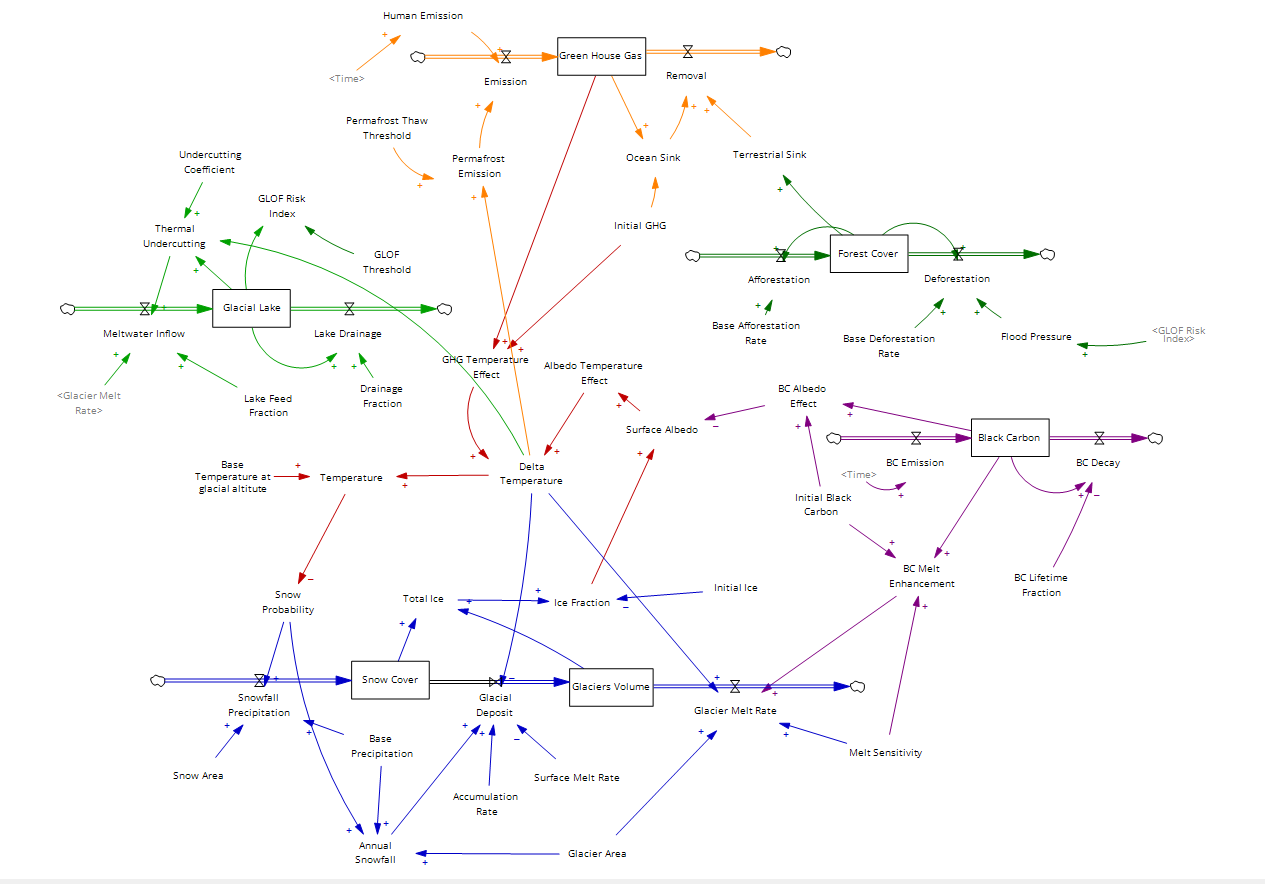
\includegraphics[width=\textwidth]{Updated_Graphs/SFD.png}
    \caption{Stock and Flow Diagram of the Nepal glacier system. Boxes represent stocks, valves represent flows, and colored arrows represent causal connections grouped by subsystem.}
    \label{fig:sfd}
\end{figure}

\subsection{Key Equations}

We highlight three equations that are central to the model's behavior.

\textbf{Equation 1: GHG Temperature Effect}

\[
\text{GHG Temperature Effect} = 3 \times \frac{\ln\left(\max\left(\frac{\text{Green House Gas}}{\text{Initial GHG}},\, 1\right)\right)}{\ln(2)}
\]

This implements the logarithmic radiative forcing relationship established by Myhre et al. \cite{myhre1998}. A climate sensitivity of 3 degrees Celsius per doubling of CO\textsubscript{2} is used, consistent with the likely range reported in IPCC AR6 \cite{ipcc2021}. At 1980 levels (830 Gt CO\textsubscript{2}), the effect is zero by construction. As GHG accumulates, temperature rises in a concave fashion, slowing down relative to the linear GHG growth. The division by $\ln(2)$ correctly normalizes the sensitivity to a per-doubling basis.

\textbf{Equation 2: Glacier Melt Rate}

\[
\text{Glacier Melt Rate} = \max\!\left(0,\; \left(\text{Melt Sensitivity} + \text{BC Melt Enhancement}\right) \times \Delta T \times \text{Glacier Area}\right)
\]

This is the primary outflow from the Glaciers Volume stock. Melt Sensitivity (0.86 km per year per degree Celsius) is calibrated from field observations at Yala and Rikha Samba glaciers by Stigter et al. \cite{stigter2021}. The BC Melt Enhancement term adds 39 percent of base sensitivity when Black Carbon is at its initial loading, consistent with ICIMOD measurements \cite{icimod2021}. Delta Temperature is the combined warming from GHG forcing and albedo feedback. Glacier Area (0.363 km\textsuperscript{2}) converts the depth-based rate to a volumetric flow. The MAX function prevents the flow from going negative, ensuring no spurious re-freezing at glacier scales.

\textbf{Equation 3: Permafrost Emission}

\[
\text{Permafrost Emission} = \begin{cases} 0.0154 \times (\Delta T - 1.5) & \text{if } \Delta T > 1.5 \\ 0 & \text{otherwise} \end{cases}
\]

The coefficient 0.0154 Gt CO\textsubscript{2} per degree Celsius per year is derived from Schuur et al. \cite{schuur2015}, who estimate approximately 0.9 Gt CO\textsubscript{2} per degree of warming per year globally from permafrost thaw. We apply a Hindu Kush Himalaya fraction of roughly 1.7 percent to obtain the Nepal-relevant contribution. The threshold of 1.5 degrees Celsius represents the warming level at which permafrost thaw transitions from negligible to significant in this region.

\subsection{Parameter Table}

\begin{table}[H]
    \centering
    \renewcommand{\arraystretch}{1.3}
    \begin{tabular}{|p{4.5cm}|p{2.2cm}|p{2.2cm}|p{5.5cm}|}
        \hline
        \textbf{Parameter} & \textbf{Value} & \textbf{Unit} & \textbf{Source} \\
        \hline
        Initial GHG & 830 & Gt CO\textsubscript{2} & IPCC AR6 \cite{ipcc2021} \\
        Initial Glaciers Volume & 312 & km\textsuperscript{3} & ICIMOD HI-WISE \cite{icimod2023} \\
        Initial Snow Cover & 50 & km\textsuperscript{3} & Brun et al. \cite{brun2017} \\
        Initial Glacial Lake & 0.5 & km\textsuperscript{3} & Rounce et al. \cite{rounce2020} \\
        Initial Forest Cover & 64,000 & km\textsuperscript{2} & Global Forest Watch \cite{gfw2024} \\
        Initial Black Carbon & 120 & Gg & ICIMOD \cite{icimod2021} \\
        Base Temperature at glacial altitude & $-15$ & Celsius & World Bank Nepal \cite{worldbank2021} \\
        Melt Sensitivity & 0.86 & km/yr & Stigter et al. \cite{stigter2021} \\
        Accumulation Rate & 0.55 & dimensionless & Stigter et al. \cite{stigter2021} \\
        Permafrost Thaw Threshold & 1.5 & $^\circ$C ($\Delta T$) & Schuur et al. \cite{schuur2015} \\
        Permafrost Coefficient & 0.0154 & Gt CO\textsubscript{2}/($^\circ$C yr) & Schuur et al. \cite{schuur2015} \\
        Ocean Sink Coefficient & 10.6 & Gt CO\textsubscript{2}/yr & Friedlingstein et al. \cite{friedlingstein2022} \\
        Lake Feed Fraction & 0.3 & dimensionless & Rounce et al. \cite{rounce2020} \\
        Glacier Area & 0.363 & km\textsuperscript{2} & ICIMOD \cite{icimod2023} \\
        BC Lifetime Fraction & 0.5 & 1/yr & ICIMOD \cite{icimod2021} \\
        Base Afforestation Rate & 0.014 & 1/yr & Global Forest Watch \cite{gfw2024} \\
        Base Deforestation Rate & 0.012 & 1/yr & Global Forest Watch \cite{gfw2024} \\
        GLOF Threshold & 5 & km\textsuperscript{3} & ICIMOD \cite{icimod2023} \\
        \hline
    \end{tabular}
    \caption{Key model parameters, their values, units, and sources.}
    \label{tab:params}
\end{table}

\subsection{Model Testing}

Before running policy scenarios, we performed two basic structural tests in Vensim. First, we confirmed that both ``Units are OK'' and ``Model is OK'' checks passed with no errors. Second, we tested boundary behavior by setting Delta Temperature to zero for the entire simulation. In this case, Glacier Melt Rate collapses to zero and Glaciers Volume rises gradually as Glacial Deposit continues to add compacted snowfall. This is the physically expected behavior: with no warming, glaciers would slowly accumulate mass. Third, we set Human Emission to zero, confirming that GHG stock drops monotonically as ocean and terrestrial sinks continue removing pre-existing carbon. These tests give us confidence that the model's causal structure is internally consistent.

% ============================================================
\section{Policy Analysis and Results}
% ============================================================

\subsection{Base Case}

The base case uses all default parameter values with Human Emission growth at 1.8 percent per year (historical average from Global Carbon Project \cite{gcp2022}) and Black Carbon emissions growing at 1.2 percent per year \cite{icimod2021}. Figure \ref{fig:ghg_base} shows GHG accumulation rising from 830 Gt CO\textsubscript{2} in 1980 to approximately 8,395 Gt CO\textsubscript{2} by 2080 under the base case, a tenfold increase driven by exponential emission growth that far outpaces the logarithmically saturating ocean sink.

\begin{figure}[H]
    \centering
    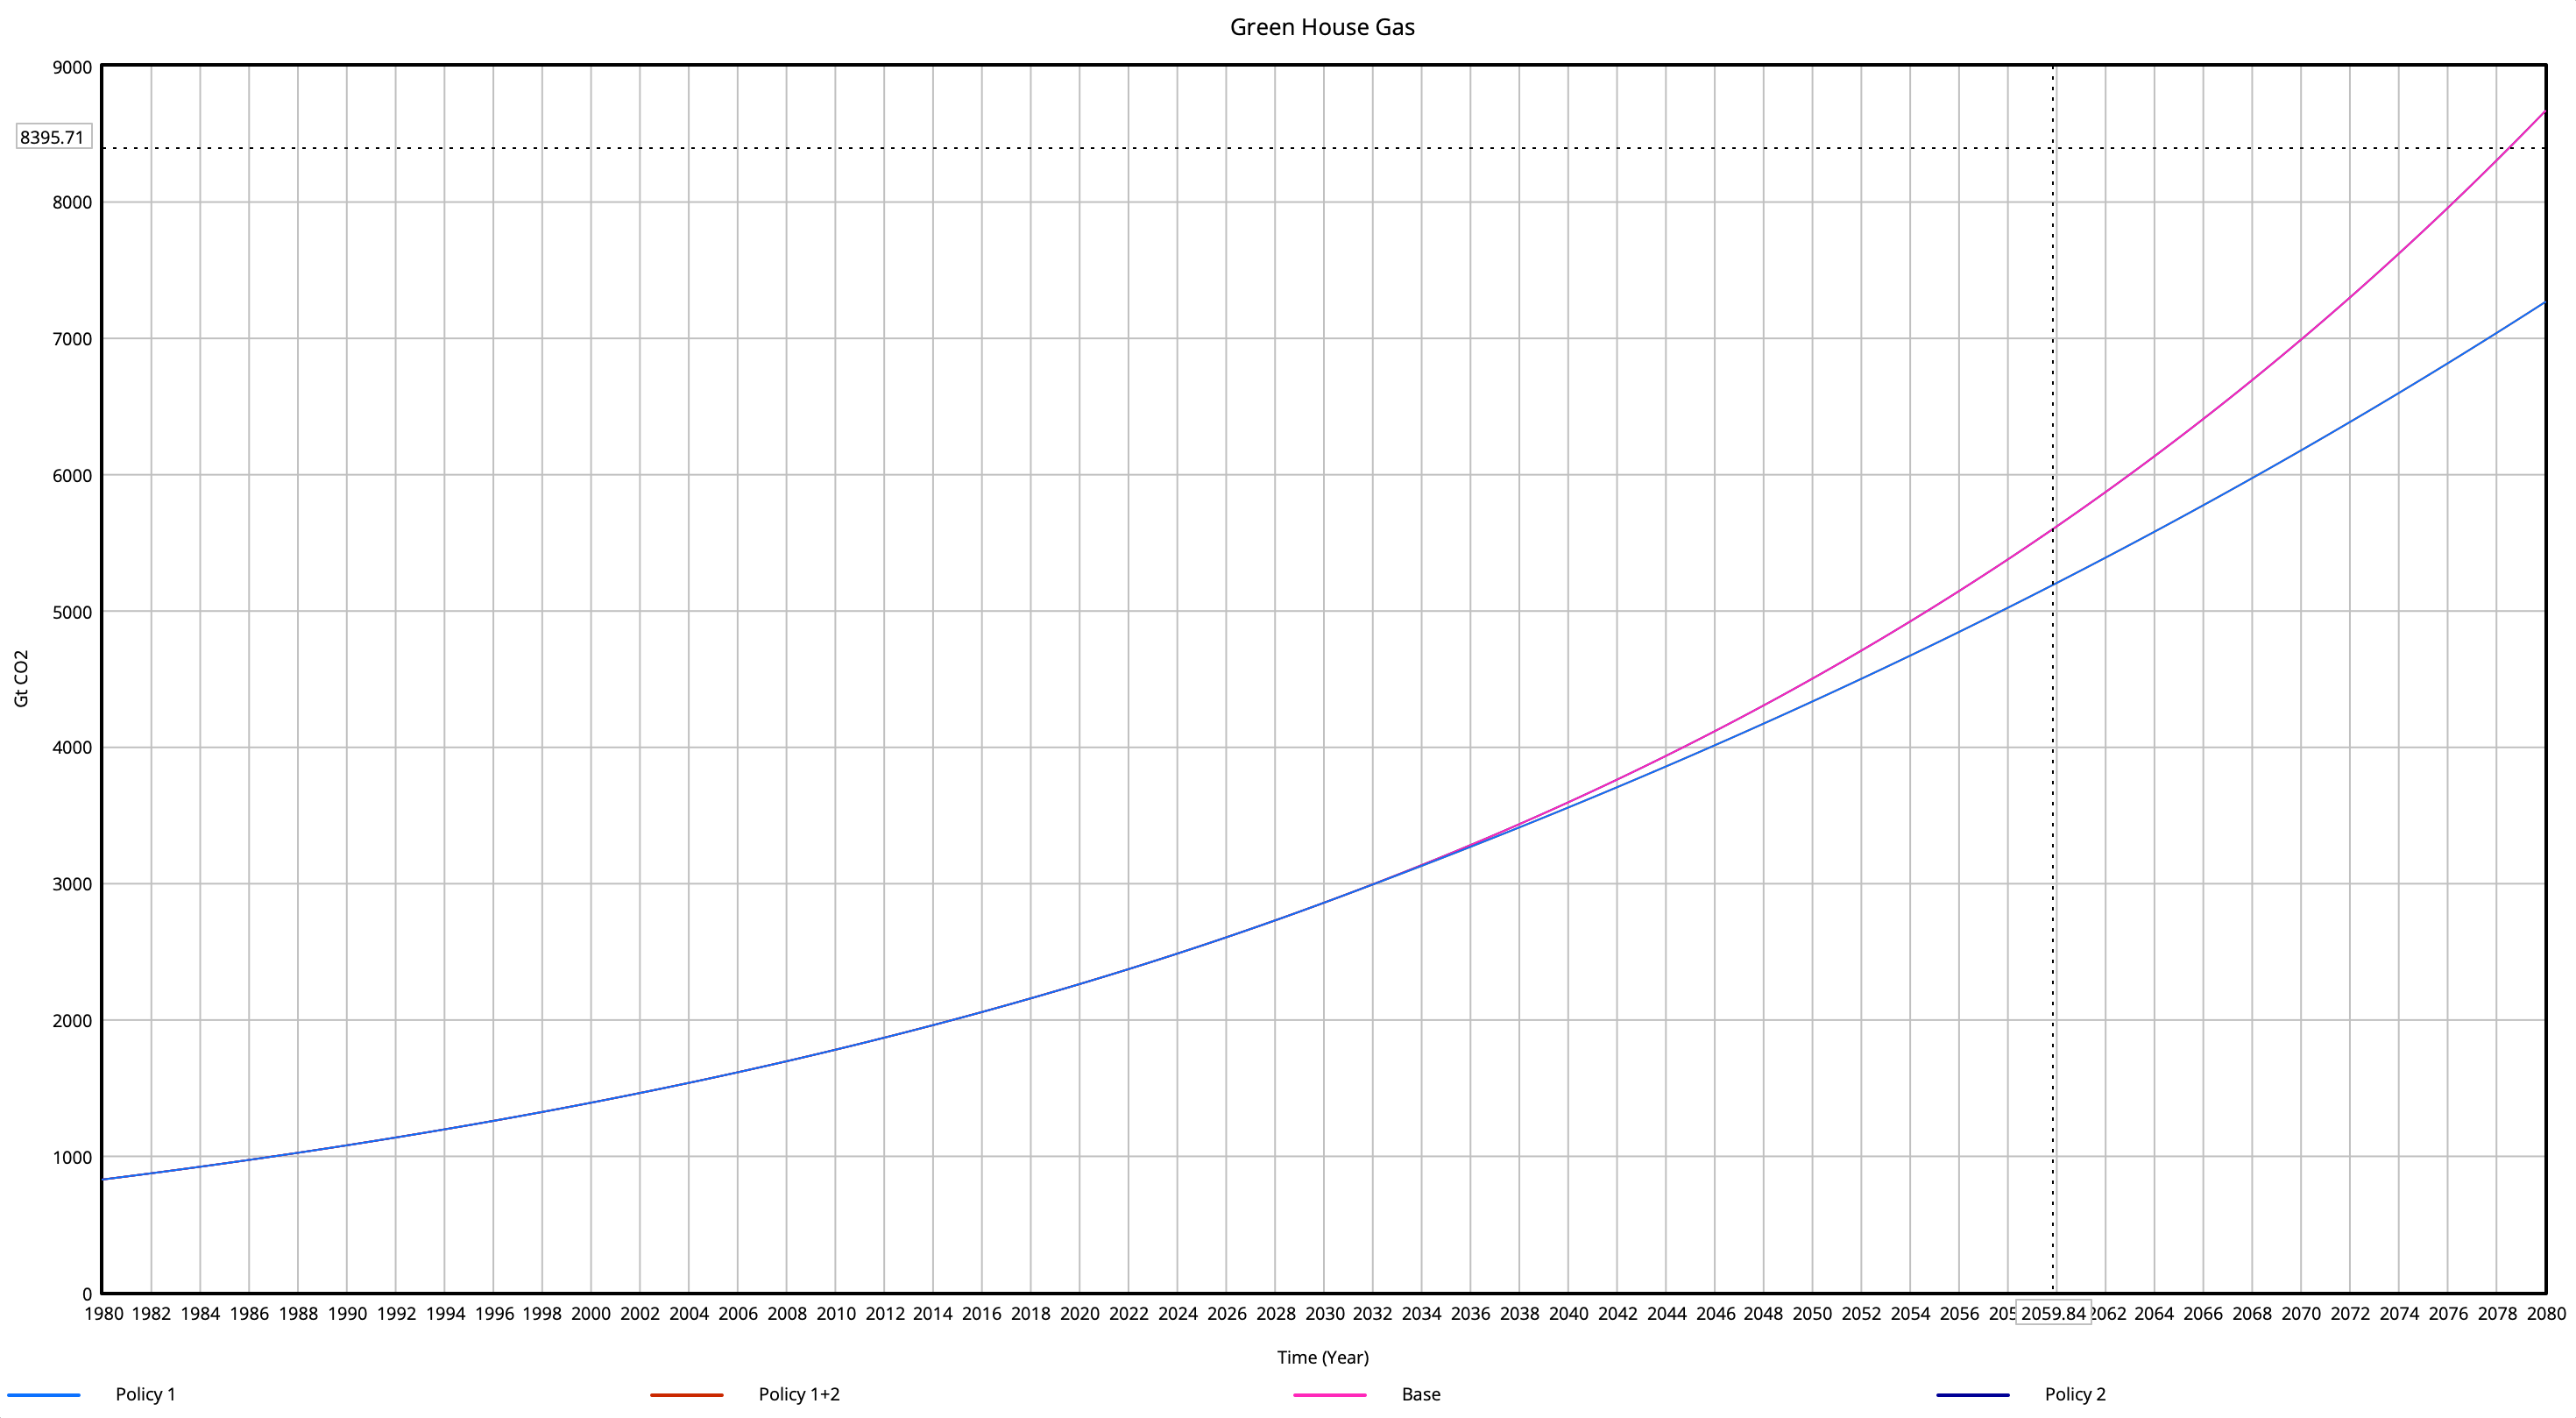
\includegraphics[width=0.9\textwidth]{Updated_Graphs/Graphs_for_policy_1&2/GHG.png}
    \caption{Green House Gas stock (Gt CO\textsubscript{2}) from 1980 to 2080. The base case (pink) reaches approximately 8,395 Gt CO\textsubscript{2} by 2080. Policy 1 (light blue, emission growth reduction) substantially lowers GHG accumulation. Policy 2 (dark blue, BC reduction) and the combined scenario (red) show intermediate trajectories.}
    \label{fig:ghg_base}
\end{figure}

Temperature at glacier altitude rises from approximately $-14.7^\circ$C in 1980 to $-8.2^\circ$C by 2080 in the base case, representing roughly 6.5 degrees of warming over the century. As a result, Glaciers Volume falls from 312 km\textsuperscript{3} to approximately 155 km\textsuperscript{3}, a loss of 50 percent of the 1980 baseline. The GLOF Risk Index, which starts near zero in 1980 as lake volumes are small, grows continuously and reaches 0.68 by 2080, indicating the aggregate glacial lake system is approaching two thirds of the critical volume threshold. Black Carbon grows from 120 Gg at the 1980 equilibrium to approximately 334 Gg by 2080 as South Asian emissions continue rising.

\subsection{Sensitivity Analysis}

To assess model robustness, we analytically evaluated the effect of a 20 percent change in two key parameters.

\textbf{Melt Sensitivity ($\pm$20\%):} Melt Sensitivity enters the Glacier Melt Rate equation multiplicatively alongside Delta Temperature and Glacier Area. A 20 percent increase (from 0.86 to 1.032 km per year per degree Celsius) therefore increases Glacier Melt Rate proportionally at every time step. Over 100 years, this translates to a faster depletion of Glaciers Volume by an additional 15 to 20 km\textsuperscript{3} relative to the base case. Conversely, a 20 percent reduction (0.86 to 0.688) slows melt and retains approximately 15 additional km\textsuperscript{3} by 2080. Because Melt Sensitivity also feeds into BC Melt Enhancement (which scales proportionally to it), the BC albedo loop is correspondingly amplified or dampened, adding a secondary effect through the temperature pathway.

\textbf{Human Emission initial value ($\pm$20\%):} A 20 percent increase in 1980 emissions (from 36 to 43.2 Gt CO\textsubscript{2} per year) shifts the GHG trajectory upward from the first year, reaching a higher plateau by 2080 and bringing forward the crossing of the 1.5 degree permafrost threshold by several years. This activates the R3 permafrost loop earlier, causing a steeper acceleration of warming in the second half of the simulation. A 20 percent reduction delays the permafrost threshold crossing and reduces the terminal GHG stock by roughly 800 Gt CO\textsubscript{2} by 2080. The sensitivity to this parameter confirms that early action on emission reductions delivers compounding benefits through the permafrost feedback pathway.

\subsection{Policy 1: Human Emission Growth Rate Reduction}

This policy reduces the emission growth rate from 1.8 percent per year to 1.0 percent per year starting in 2030, representing a moderate decarbonization trajectory consistent with the IEA Stated Policies Scenario \cite{iea2021}. Emissions still grow, but more slowly. The effect on GHG accumulation is substantial: by 2080, GHG reaches approximately 7,300 Gt CO\textsubscript{2} rather than 8,395 Gt CO\textsubscript{2}, a difference of roughly 1,100 Gt CO\textsubscript{2}. This moderates the GHG Temperature Effect and slows warming. However, the effect on Glaciers Volume is limited, as shown in Figure \ref{fig:glacvol}. The lines for Policy 1 and the base case track closely through 2060, diverging only in the final two decades. By 2080, Policy 1 retains approximately 163 km\textsuperscript{3} compared to 155 km\textsuperscript{3} in the base case, a modest improvement of 8 km\textsuperscript{3}.

\begin{figure}[H]
    \centering
    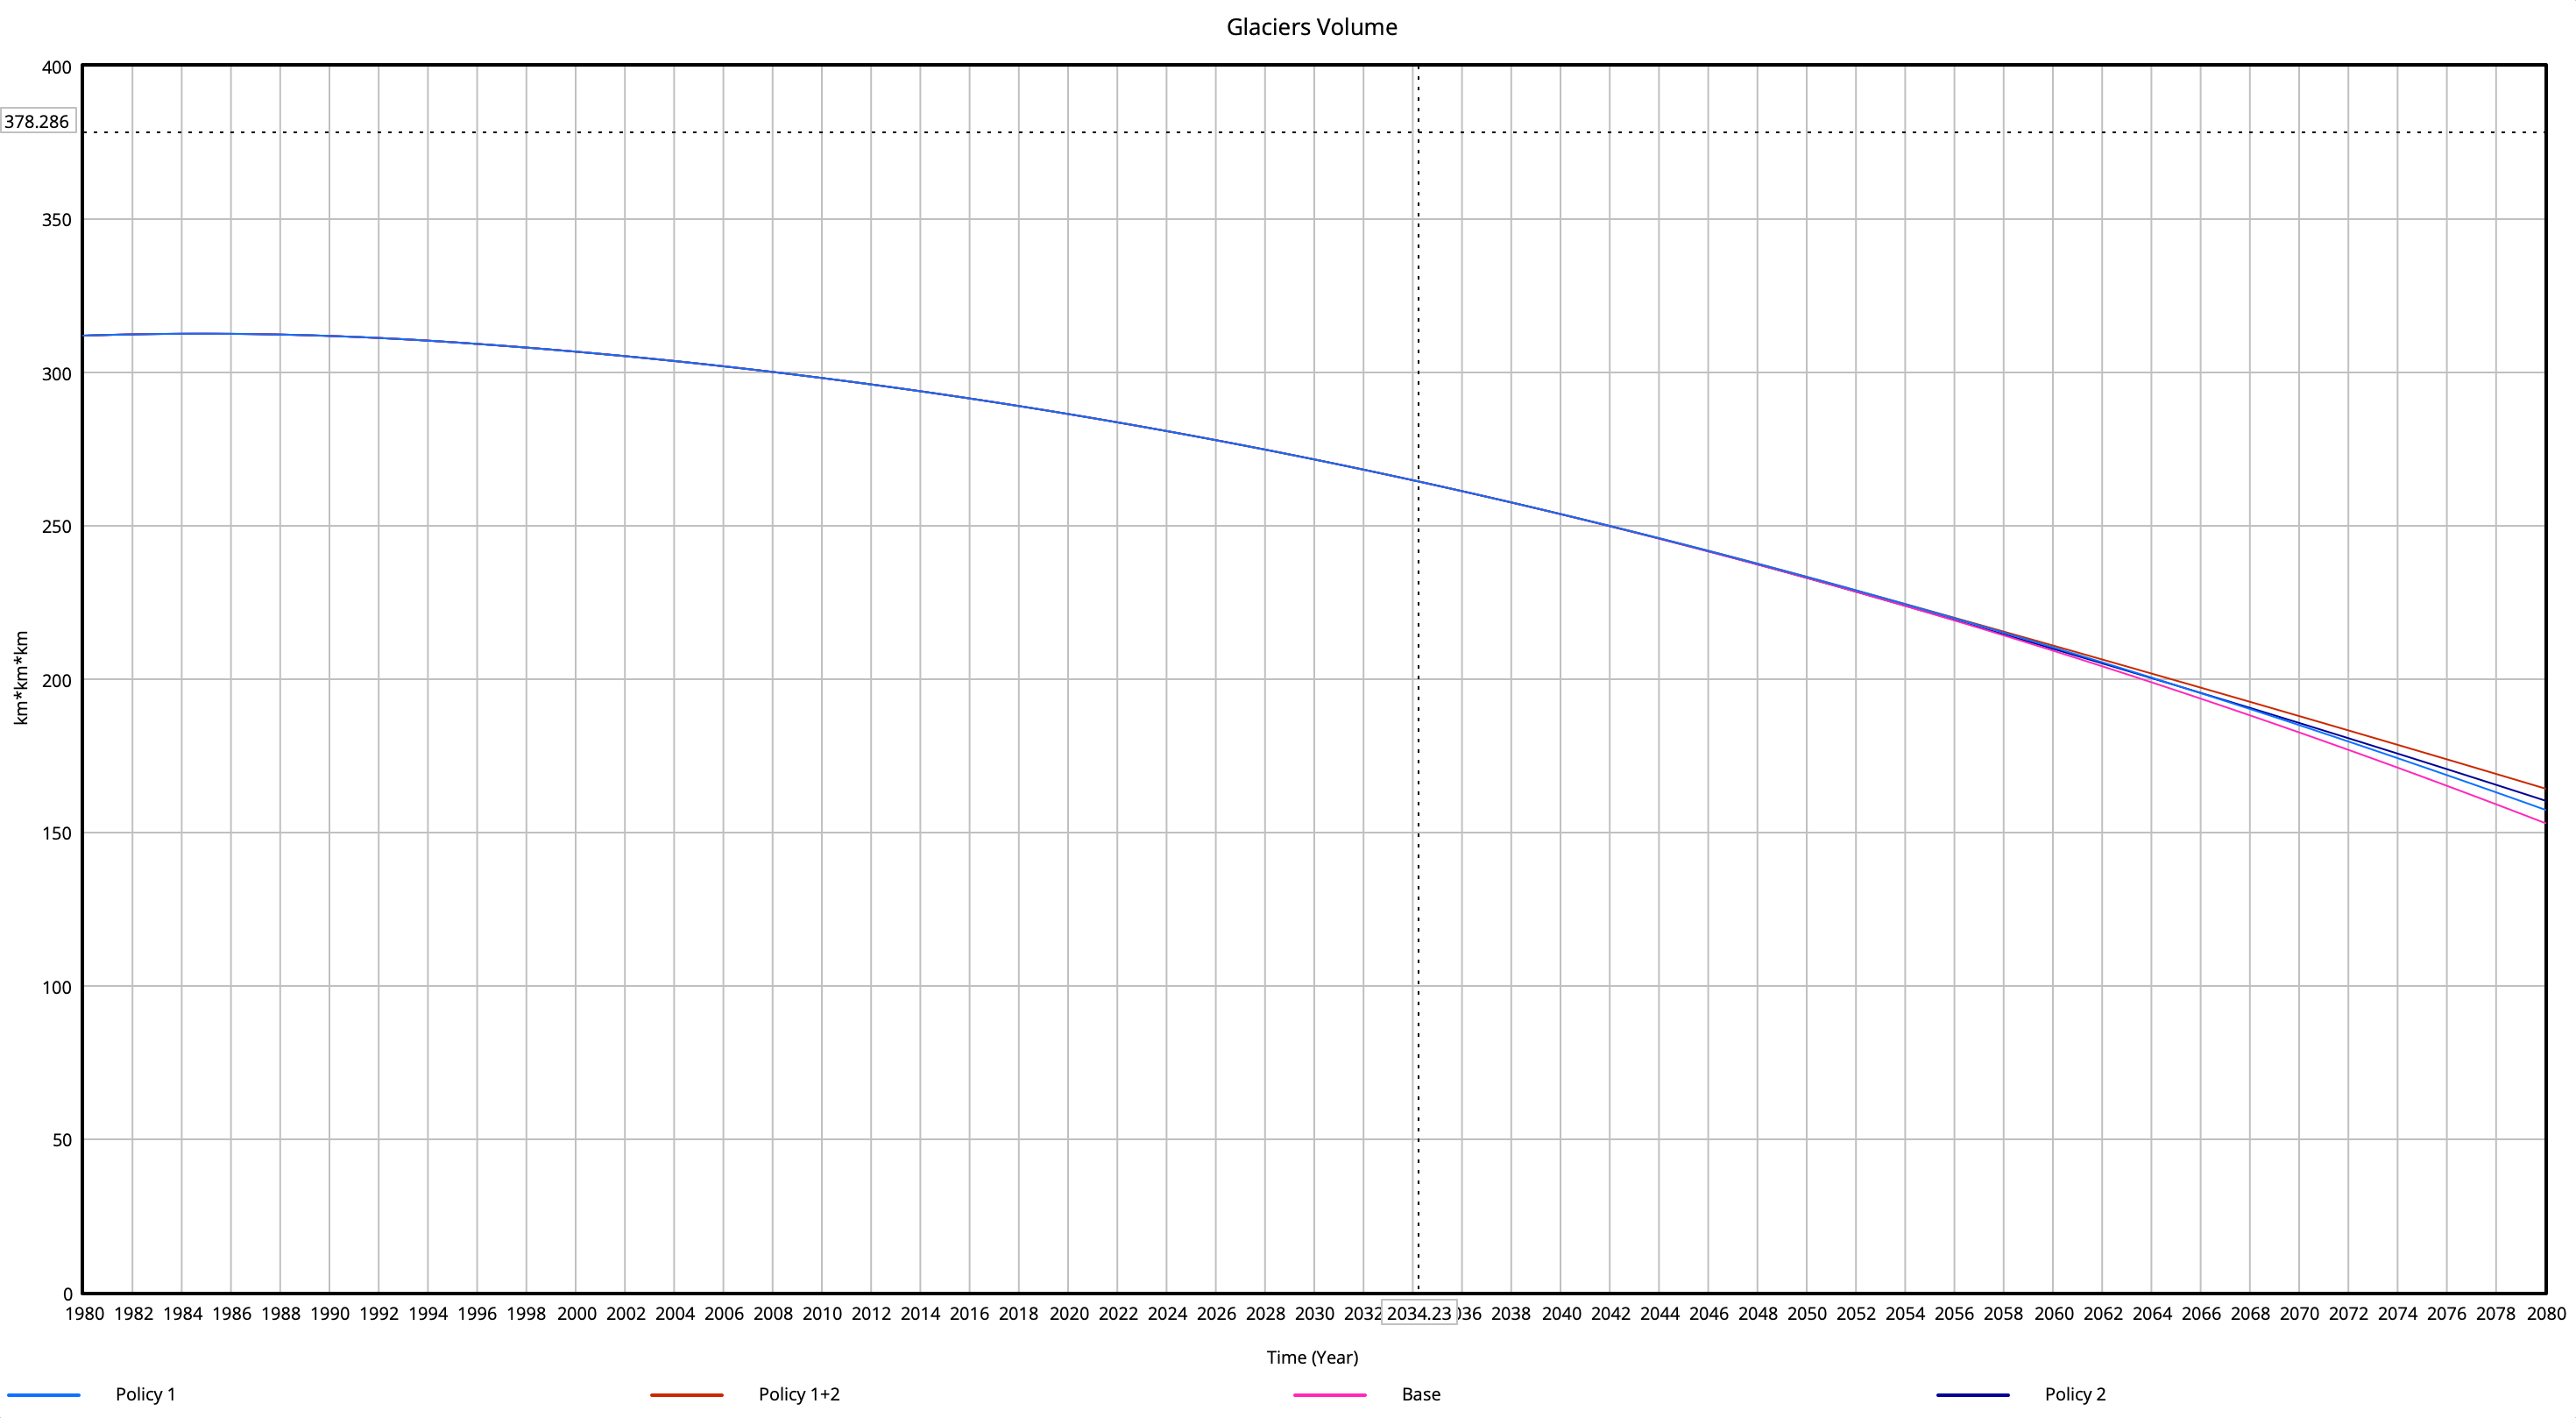
\includegraphics[width=0.9\textwidth]{Updated_Graphs/Graphs_for_policy_1&2/Glaciers Volume.png}
    \caption{Glaciers Volume (km\textsuperscript{3}) comparing base case (pink), Policy 1 (light blue, emission growth reduction), Policy 2 (dark blue, BC reduction), and combined Policy 1 plus 2 (red). Policies diverge from the base only after 2060, highlighting the inertia of the climate system.}
    \label{fig:glacvol}
\end{figure}

This limited glacier response despite a substantial GHG reduction reflects the thermal inertia of the climate system. Warming already accumulated before 2030 continues driving melt, and the temperature reduction from slower GHG growth only becomes meaningful toward the end of the century. Nevertheless, this policy delivers a long term benefit beyond 2080 as the lower GHG trajectory reduces the probability of crossing the permafrost tipping point.

\subsection{Policy 2: Black Carbon Emission Growth Rate Reversal}

This policy reverses BC emission growth from plus 1.2 percent per year to minus 3 percent per year after 2030, representing aggressive deployment of clean brick kiln technology, diesel emission standards, and elimination of crop residue burning across the Indo-Gangetic Plain. ICIMOD research suggests that a 30 to 50 percent reduction in BC is achievable within 15 years through existing technology in South Asia \cite{icimod2021}, and Bond et al. \cite{bond2013} confirm the technical feasibility of this scale of mitigation. Because BC has an atmospheric lifetime of approximately two years (BC Lifetime Fraction = 0.5 per year), the BC stock responds quickly to changes in emission rates.

Figure \ref{fig:bc} shows that Black Carbon in the base case and Policy 1 scenarios both grow continuously (overlapping light blue and pink lines), reaching over 300 Gg by 2080. Under Policy 2 and the combined scenario (Policy 1 plus 2), Black Carbon peaks around 2030 at approximately 215 Gg and then falls sharply to approximately 55 Gg by 2080.

\begin{figure}[H]
    \centering
    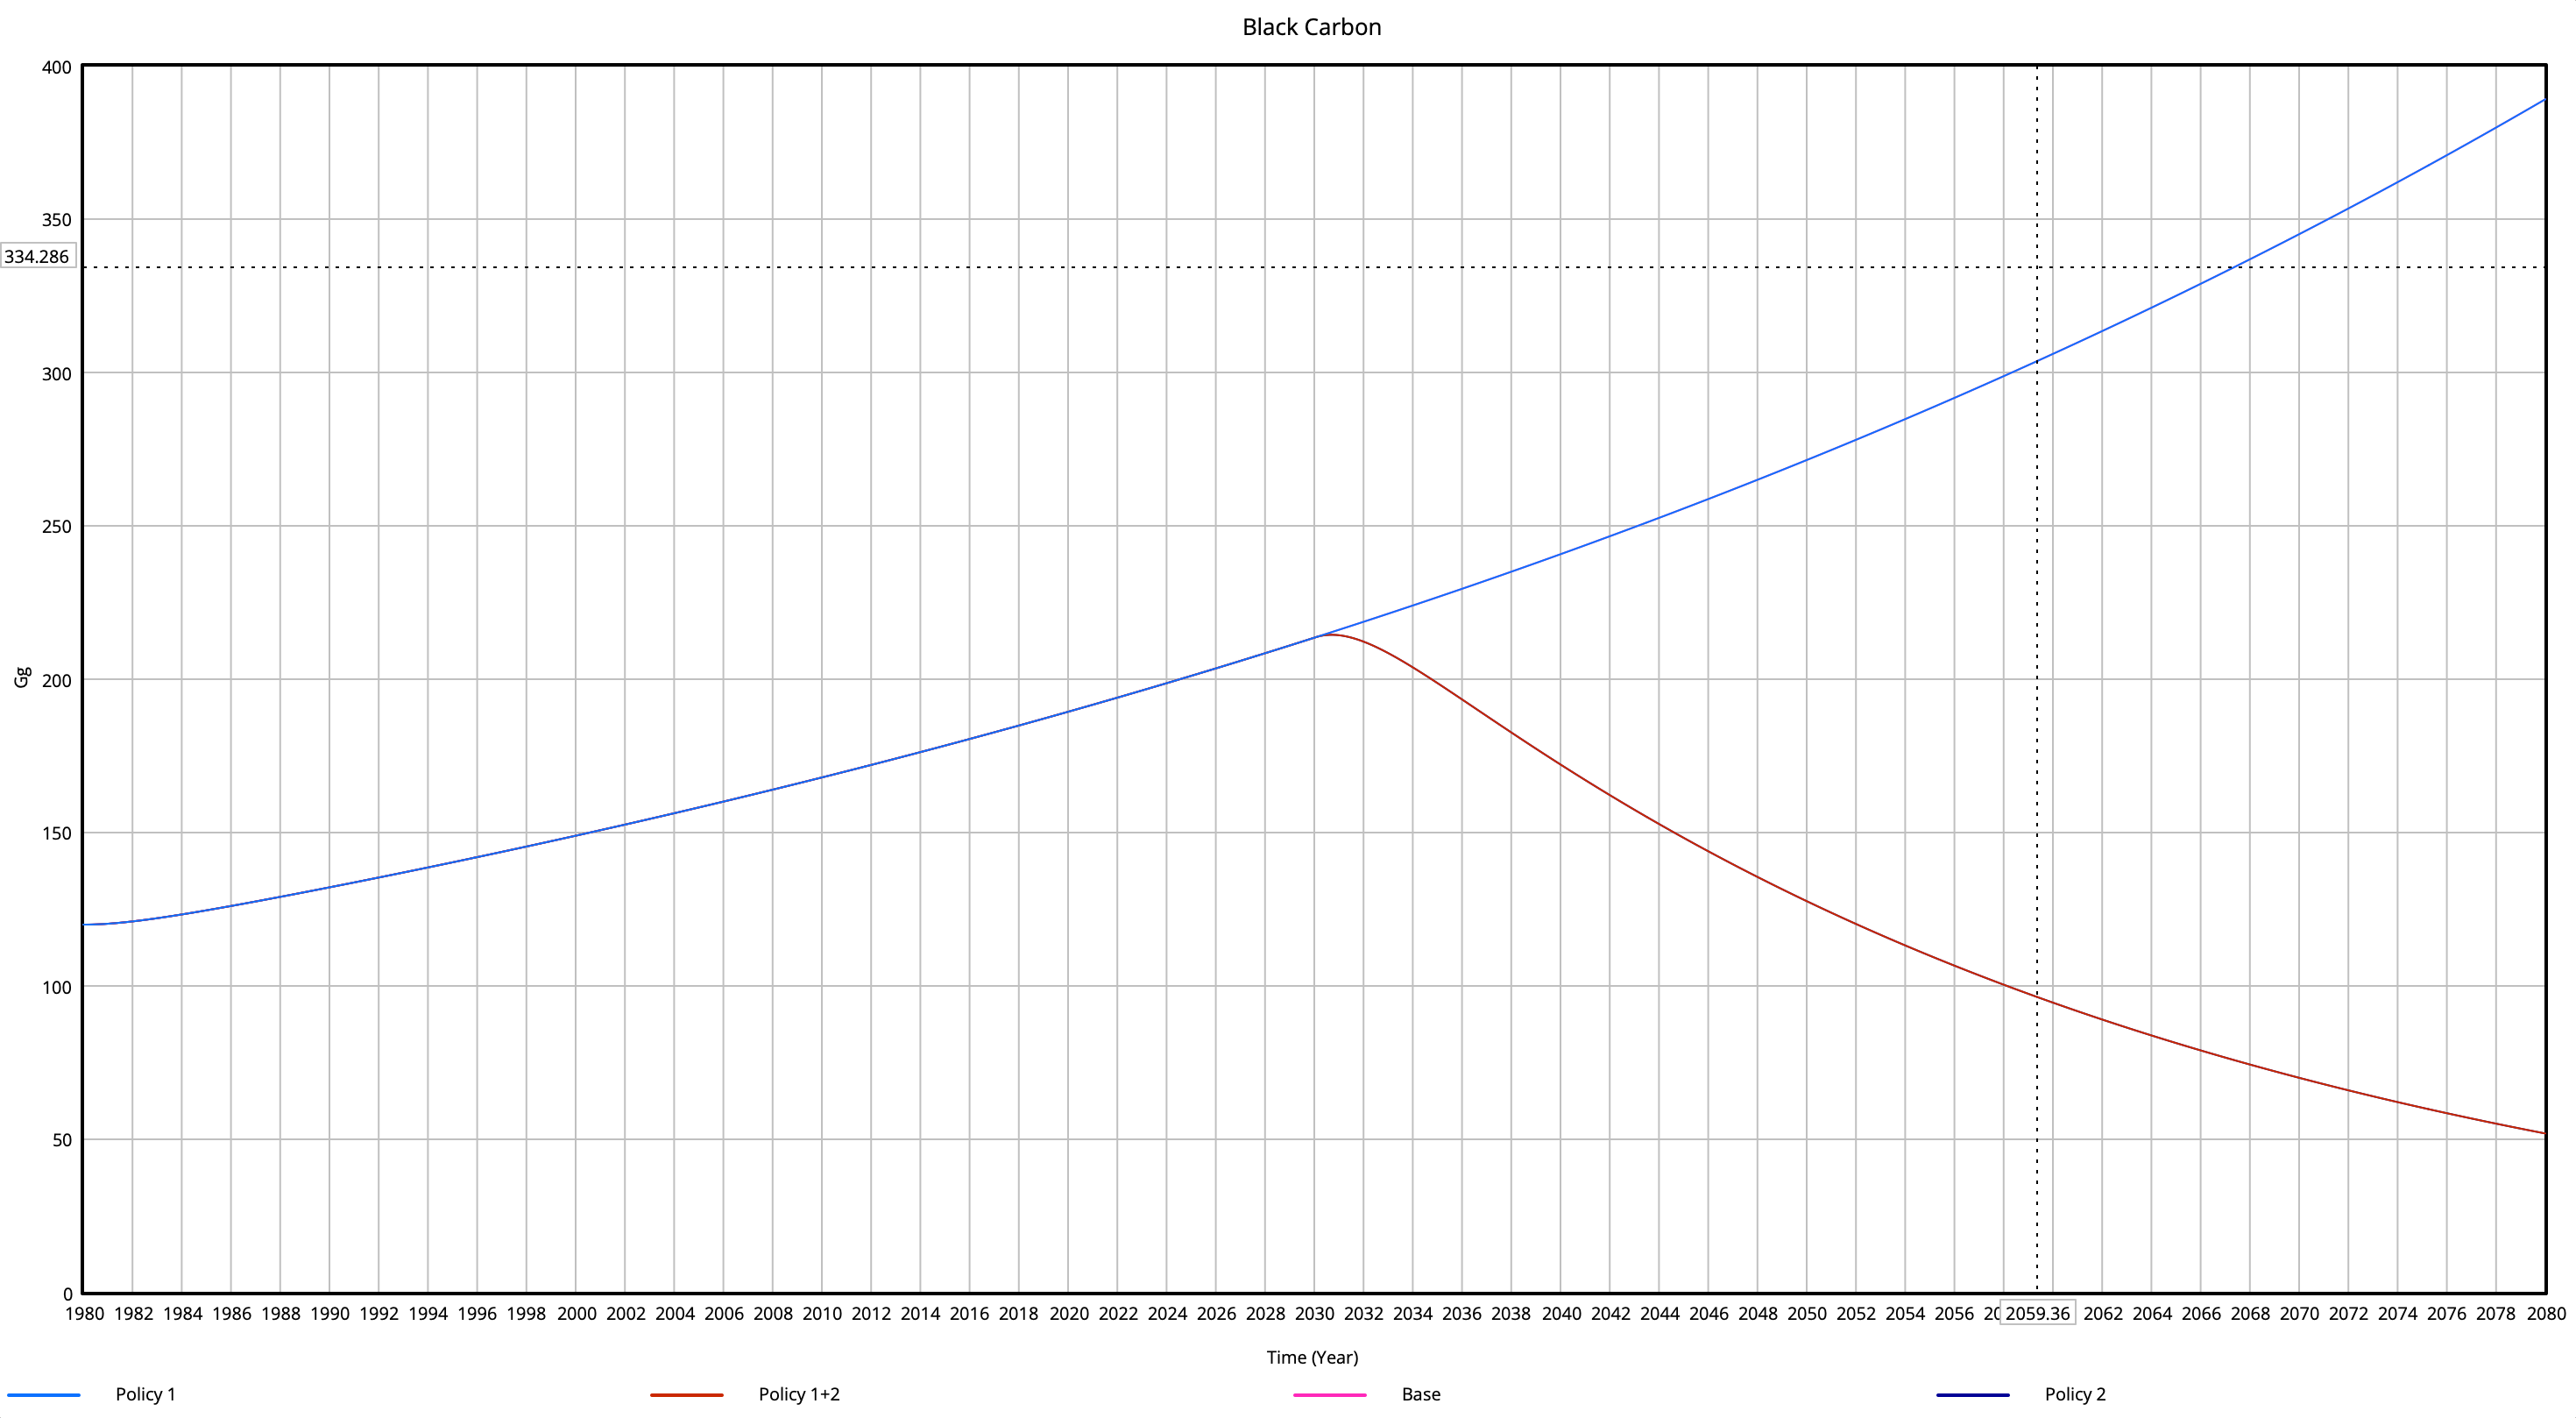
\includegraphics[width=0.9\textwidth]{Updated_Graphs/Graphs_for_policy_1&2/Black Carbon.png}
    \caption{Black Carbon stock (Gg) under all scenarios. Policy 2 (and Policy 1 plus 2, shown in red) reverses BC growth after 2030, causing the stock to fall from a peak of approximately 215 Gg to around 55 Gg by 2080. The base case and Policy 1 (which does not target BC) overlap on the rising trajectory.}
    \label{fig:bc}
\end{figure}

The most pronounced benefit of BC reduction is on the GLOF Risk Index. Figure \ref{fig:glof} shows that the base case reaches a GLOF Risk Index of 0.68 by 2080, while Policy 2 and the combined scenario reduce this to approximately 0.57. The mechanism is: lower BC reduces BC Albedo Effect, raising Surface Albedo, which reduces Albedo Temperature Effect and therefore Delta Temperature. A cooler Delta Temperature slows Glacier Melt Rate, which reduces Meltwater Inflow to the glacial lake, which slows lake growth and limits the activation of the Thermal Undercutting reinforcing loop. This is a particularly important result because GLOF events pose direct threats to infrastructure, agriculture, and human lives in Nepal's river valleys \cite{hindu2024}.

\begin{figure}[H]
    \centering
    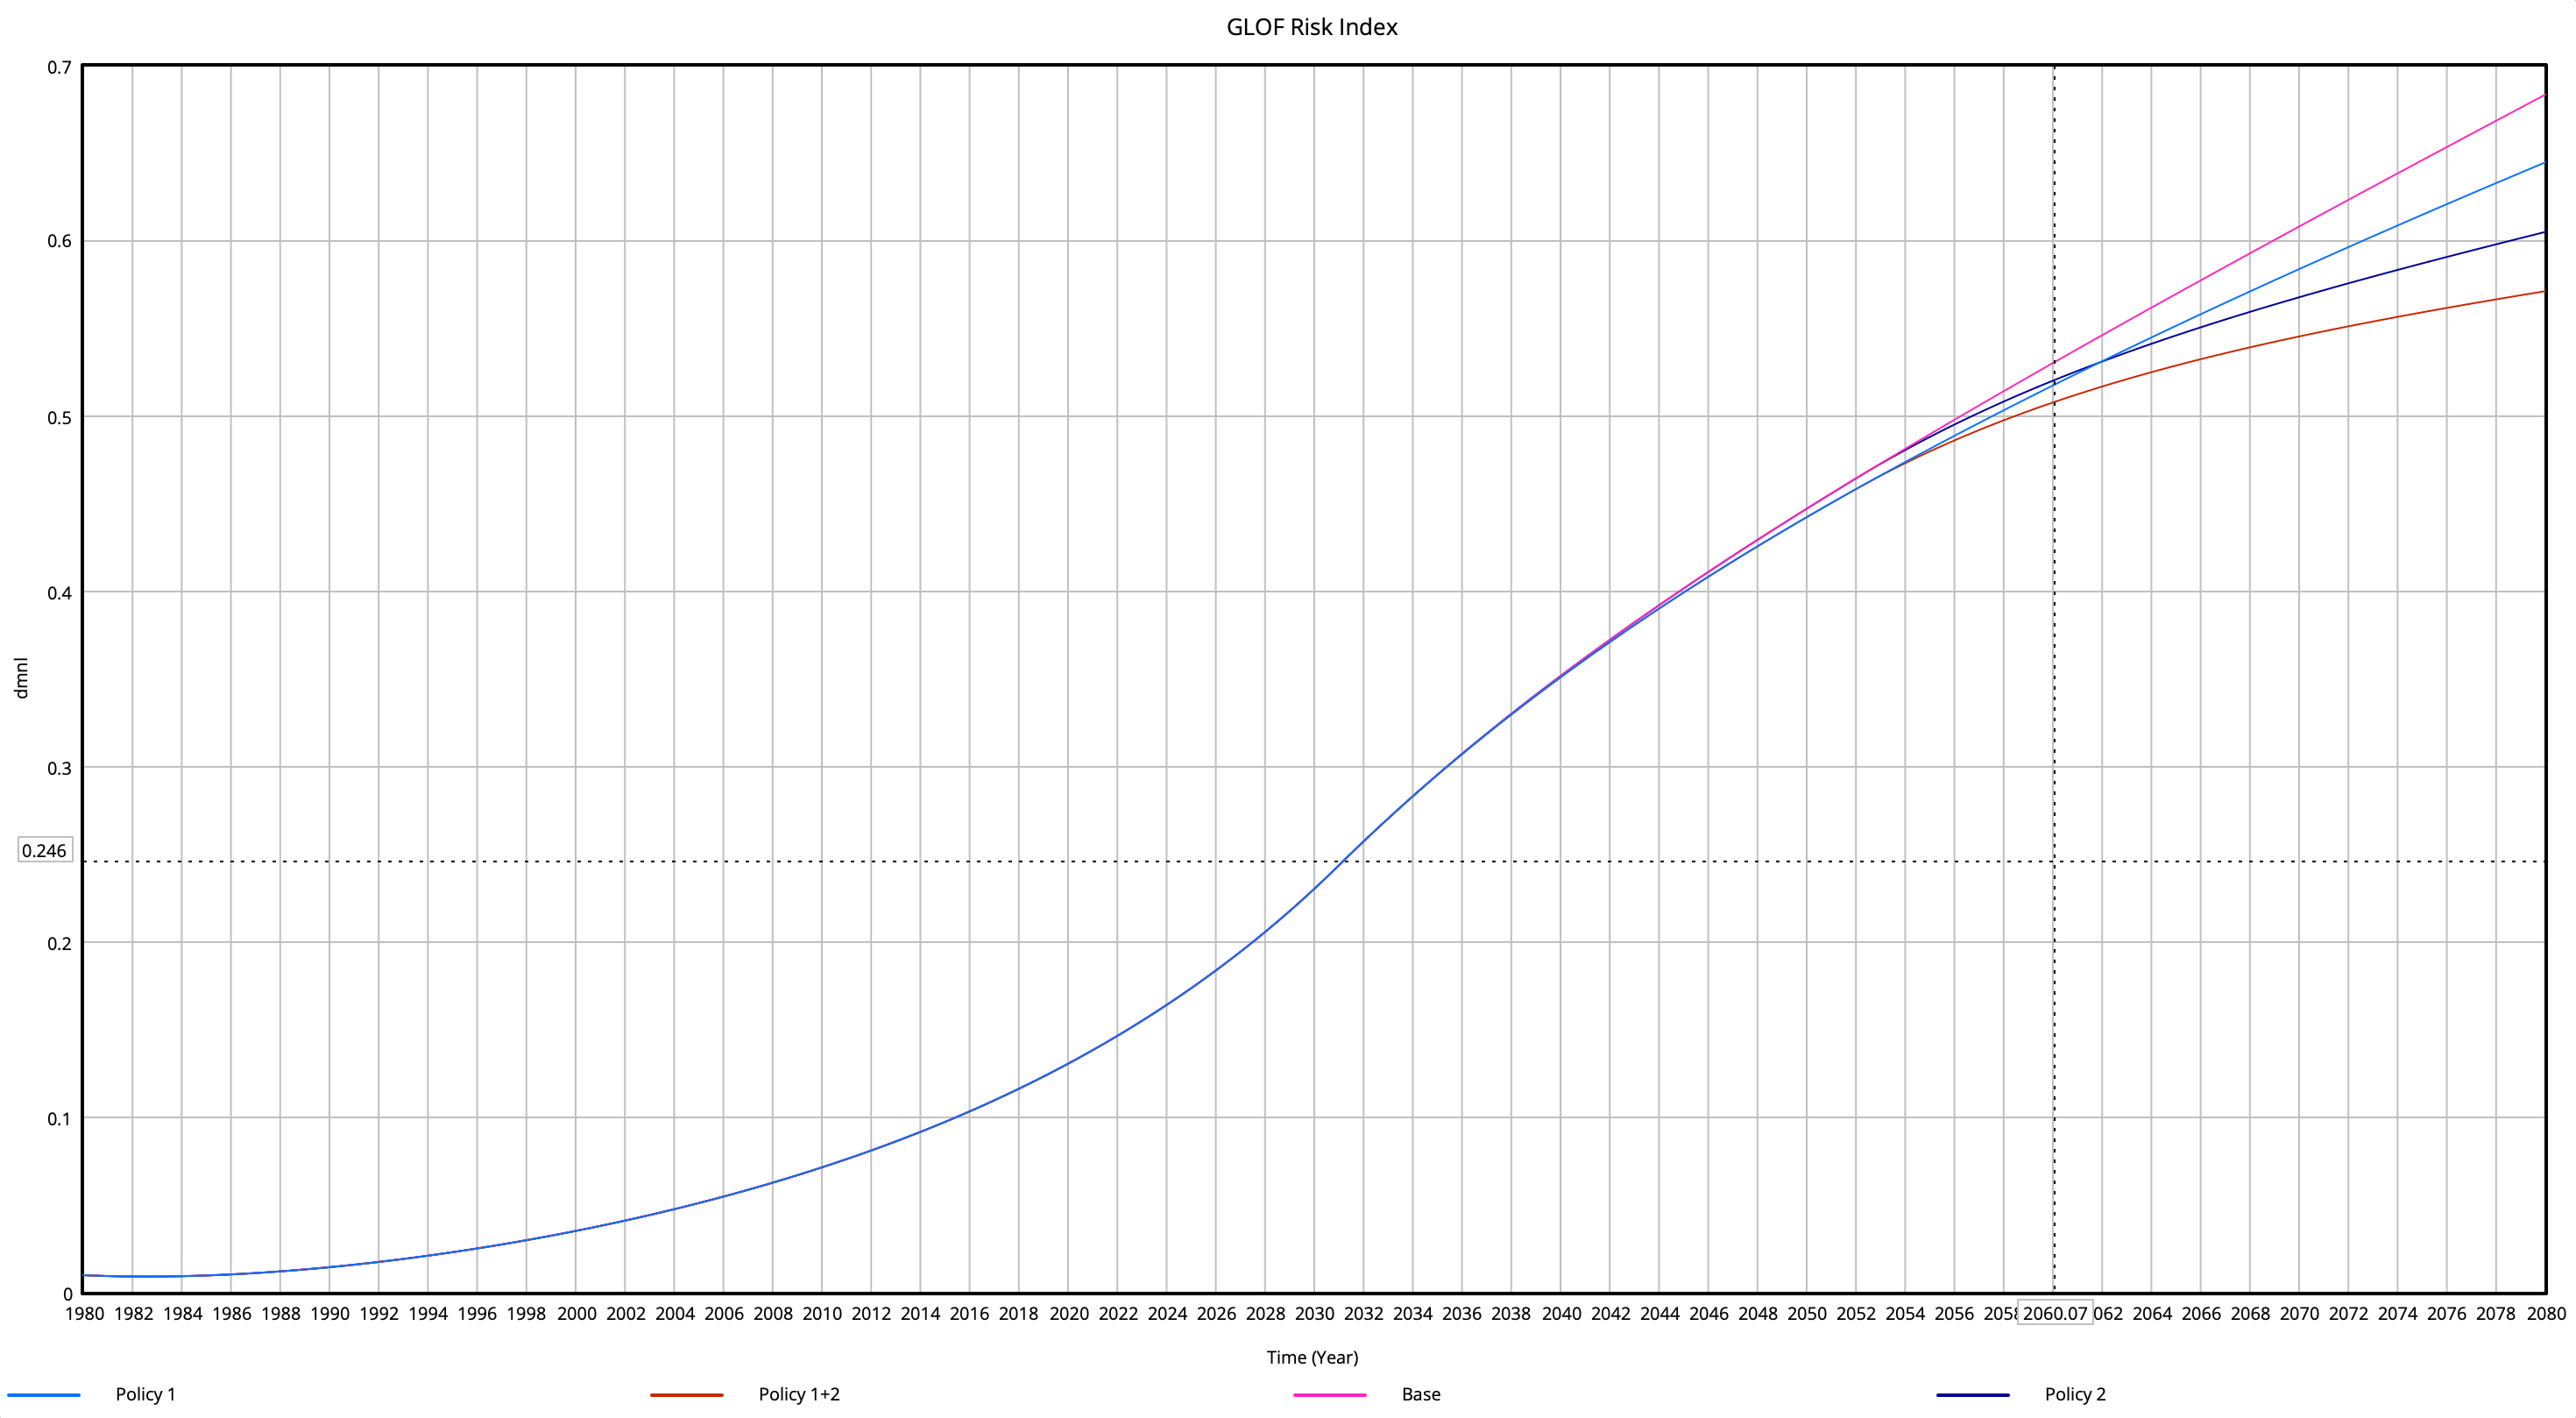
\includegraphics[width=0.9\textwidth]{Updated_Graphs/Graphs_for_policy_1&2/GLOF Risk Index.png}
    \caption{GLOF Risk Index (dimensionless, 0 to 1) from 1980 to 2080. The base case (pink) reaches 0.68 by 2080. Policy 2 and the combined scenario (red) reduce this to approximately 0.57. The index follows an accelerating growth path driven by the GLOF undercutting reinforcing loop (R2).}
    \label{fig:glof}
\end{figure}

\subsection{Bonus Exploration: Melt Sensitivity Reduction (Policy 3)}

As an exploratory extension, we examined a physical glacier protection intervention in which Melt Sensitivity is reduced from 0.86 to 0.602 km per year per degree Celsius after 2030, representing a 30 percent reduction. This simulates the partial coverage of glacier surfaces with reflective geotextile blankets, an approach that has demonstrated 50 to 70 percent melt reduction on covered areas in field experiments \cite{zenklusen2012, oerlemans2017}. The 30 percent system-level figure is conservative, reflecting the reality that only a fraction of Nepal's 3,902 km\textsuperscript{2} glacier area can realistically be covered.

\begin{figure}[H]
    \centering
    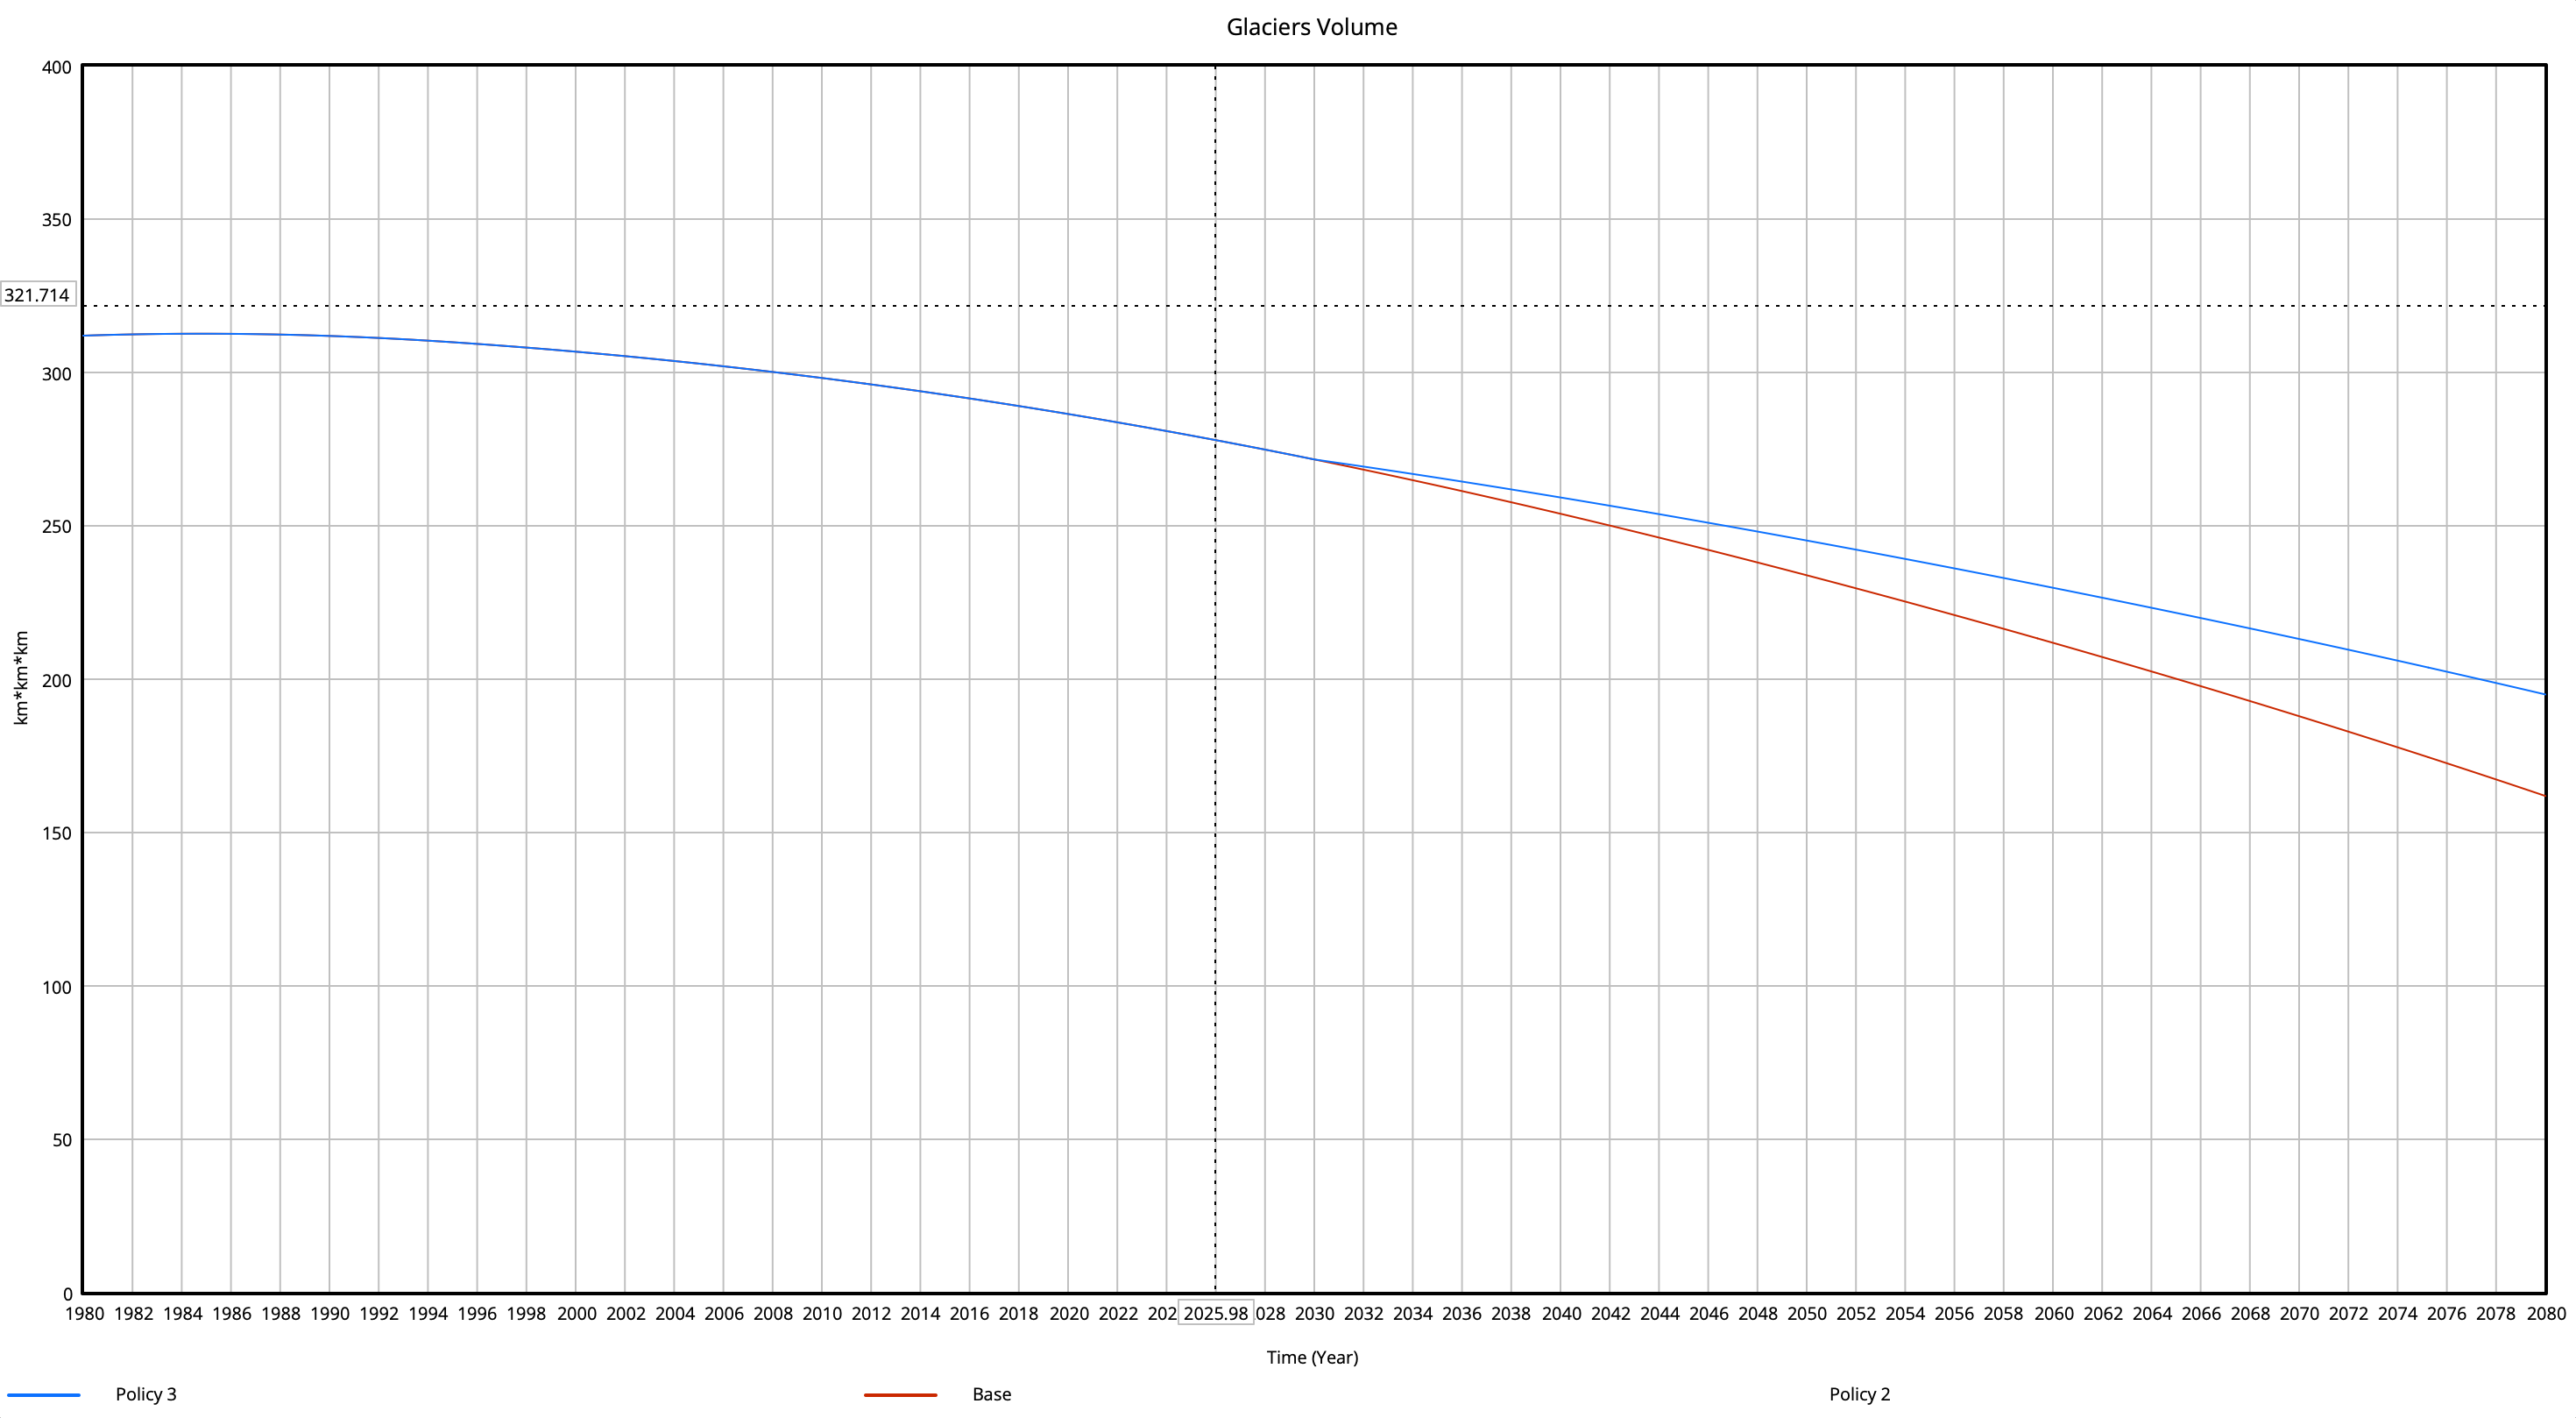
\includegraphics[width=0.9\textwidth]{Updated_Graphs/Graphs_for_policy_3/Glacier Volume.png}
    \caption{Glaciers Volume under Policy 3 (Melt Sensitivity reduction, shown in blue) versus base case (red). Policy 3 retains approximately 197 km\textsuperscript{3} by 2080, compared to 165 km\textsuperscript{3} in the base case, preserving an additional 32 km\textsuperscript{3} of glacier ice.}
    \label{fig:policy3}
\end{figure}

As Figure \ref{fig:policy3} shows, this intervention retains approximately 197 km\textsuperscript{3} of glacier ice by 2080, compared to 165 km\textsuperscript{3} in the base case, a preservation of an additional 32 km\textsuperscript{3} or roughly 19 percent more ice. This is a larger glacier volume improvement than either Policy 1 or Policy 2 achieve on their own. However, this policy was considered a bonus exploration rather than a primary recommendation because large scale physical glacier protection is extremely costly, logistically challenging across 3,902 km\textsuperscript{2} of high altitude terrain, and not scalable as a primary climate response strategy.

% ============================================================
\section{Conclusions and Recommendations}
% ============================================================

\subsection{What Happens in the Base Case}

Under business as usual conditions, the Nepal glacier system undergoes severe and accelerating degradation over the coming century. Glaciers Volume falls from 312 km\textsuperscript{3} to approximately 155 km\textsuperscript{3}, a loss of nearly half the 1980 ice mass. The GHG stock grows tenfold from 830 to over 8,000 Gt CO\textsubscript{2}. GLOF Risk Index approaches 0.68, meaning the aggregate glacial lake system accumulates more than two thirds of the critical volume associated with high outburst flood risk. This poses direct threats to the communities, infrastructure, and agriculture in Nepal's river valleys below the glacier zone. Temperature at glacier altitude warms by approximately 6.5 degrees Celsius over the century, pushing the system well past the permafrost thaw threshold and activating the R3 self-reinforcing loop in the second half of the simulation.

\subsection{Which Policy Worked Best}

For reducing GLOF risk, which is the most immediate threat to people and property, Policy 2 (black carbon reduction) performed best. It reduced the GLOF Risk Index from 0.68 to 0.57 by 2080 and slowed glacial lake growth by weakening the R4 albedo feedback loop. For long term atmospheric stabilization, Policy 1 (emission growth reduction) was more powerful, reducing GHG accumulation by over 1,100 Gt CO\textsubscript{2} by 2080. The combined scenario delivered both benefits simultaneously. Our primary recommendation is therefore to pursue the combined policy: moderate decarbonization alongside aggressive black carbon emission control. These two interventions attack the glacier melt equation from different angles: Policy 1 reduces the temperature driving force, while Policy 2 reduces the sensitivity of ice to that temperature through the albedo and melt enhancement pathways.

\subsection{Side Effects and Unintended Consequences}

One important unintended consequence appears in the forest subsystem. When GLOF Risk Index rises under the base case, Flood Pressure on forest margins increases Deforestation, which reduces Forest Cover and weakens the already small terrestrial carbon sink. This creates a secondary reinforcing path: more melt leads to more GLOF risk, which leads to more deforestation, which reduces carbon removal, which slightly increases GHG accumulation. While the magnitude of this effect is negligible at Nepal's sequestration scale relative to global emissions, it illustrates how policies that reduce GLOF risk (such as Policy 2) also deliver a forest protection co-benefit. This co-benefit is currently undervalued in climate policy discussions focused only on emissions.

A second observation is that the BC reduction policy, despite dramatically reducing the Black Carbon stock by 2080, delivers only a modest improvement in Glaciers Volume compared to its strong effect on GLOF risk. This is because BC affects melt through the albedo pathway, which is secondary to the direct temperature-melt relationship at the glacier scale. Policymakers should therefore frame BC mitigation as a GLOF risk and water security intervention rather than purely as a glacier preservation measure.

\subsection{Learning and Inferences}

The most important learning from this modeling exercise is that the climate system's inertia means that policies implemented in 2030 show limited effect on glacier outcomes before 2060. This creates a dangerous illusion: a policy may appear ineffective in the short run while delivering significant long term divergence from the base case. The system dynamics framing makes this delay explicit through the stock accumulation structure, which conventional scenario analyses often obscure. The second major inference is that reinforcing feedback loops, particularly R1 and R2, are the primary amplifiers of glacier loss and that breaking either loop yields benefits across the entire system. Reducing black carbon disrupts both R4 and, indirectly, R2, making it a highly leveraged intervention relative to its implementation cost.

\clearpage
\section*{References}
\addcontentsline{toc}{section}{References}

\begin{thebibliography}{99}

\bibitem{ipcc2021} IPCC (2021). \textit{Climate Change 2021: The Physical Science Basis. Contribution of Working Group I to the Sixth Assessment Report of the Intergovernmental Panel on Climate Change}. Cambridge University Press.

\bibitem{myhre1998} Myhre, G., Highwood, E.J., Shine, K.P., and Stordal, F. (1998). New estimates of radiative forcing due to well mixed greenhouse gases. \textit{Geophysical Research Letters}, 25(14), 2715--2718.

\bibitem{schuur2015} Schuur, E.A.G., McGuire, A.D., Schadel, C., et al. (2015). Climate change and the permafrost carbon feedback. \textit{Nature}, 520(7546), 171--179.

\bibitem{friedlingstein2022} Friedlingstein, P., et al. (2022). Global Carbon Budget 2022. \textit{Earth System Science Data}, 14, 4811--4900.

\bibitem{icimod2023} ICIMOD (2023). \textit{Water, Ice, Society, Ecosystems in the Hindu Kush Himalaya: HI-WISE Report}. Kathmandu: ICIMOD.

\bibitem{maurer2021} Maurer, J.M., et al. (2021). Accelerated mass loss of Himalayan glaciers since the Little Ice Age. \textit{Scientific Reports}.

\bibitem{stigter2021} Stigter, E.E., et al. (2021). Mass balances of Yala and Rikha Samba glaciers, Nepal, 2000 to 2017. \textit{Earth System Science Data}, 13, 3791--3818.

\bibitem{brun2017} Brun, F., Berthier, E., Wagnon, P., Kaab, A., and Treichler, D. (2017). A spatially resolved estimate of High Mountain Asia glacier mass balances from 2000 to 2016. \textit{Nature Geoscience}, 10(9), 668--673.

\bibitem{bolch2012} Bolch, T., et al. (2012). The State and Fate of Himalayan Glaciers. \textit{Science}, 336(6079), 310--314.

\bibitem{rounce2020} Rounce, D.R., et al. (2020). Glacier ice thickness estimates for the Himalaya. \textit{Proceedings of the National Academy of Sciences}, 117(16).

\bibitem{sherpa2020} Sherpa, S.F., et al. (2020). Precipitation characteristics on Mt. Everest. \textit{One Earth}, 3(5).

\bibitem{icimod2021} ICIMOD (2021). Black carbon and other drivers of Arctic and High Mountain Asia cryosphere change. Kathmandu: ICIMOD.

\bibitem{bond2013} Bond, T.C., et al. (2013). Bounding the role of black carbon in the climate system: A scientific assessment. \textit{Journal of Geophysical Research: Atmospheres}, 118(11), 5380--5552.

\bibitem{pmc2024} Nepal Forest Carbon Project (2024). Carbon sequestration in Nepal private forests. \textit{PMC}.

\bibitem{gfw2024} Global Forest Watch (2024). Nepal forest cover dashboard. Retrieved from globalforestwatch.org.

\bibitem{hindu2024} The Hindu (2024). Himalayan glacial lakes saw 10.81 percent area expansion from 2011 to 2024.

\bibitem{worldbank2021} World Bank (2021). \textit{Nepal Climate Profile}. worldbank.org.

\bibitem{gcp2022} Global Carbon Project (2022). Global Carbon Budget 2022. Retrieved from globalcarbonproject.org.

\bibitem{iea2021} International Energy Agency (2021). \textit{Net Zero by 2050: A Roadmap for the Global Energy Sector}. Paris: IEA.

\bibitem{zenklusen2012} Zenklusen Mutter, E. and Phillips, M. (2012). Quantifying the impact of snow surface temperature inversions on energy balance and melt. \textit{Cold Regions Science and Technology}, 76--77, 8--13.

\bibitem{oerlemans2017} Oerlemans, J., et al. (2017). Estimating the roughness of a glacier surface. \textit{The Cryosphere}, 11, 2563--2576.

\bibitem{sterman2000} Sterman, J.D. (2000). \textit{Business Dynamics: Systems Thinking and Modeling for a Complex World}. McGraw-Hill.

\end{thebibliography}

% ============================================================
\appendix
\section{Full Equation List (Exported from Vensim Model)}

\begin{verbatim}
Green House Gas = INTEG(Emission - Removal, 830)
    ~ Gt CO2

Emission = Human Emission + Permafrost Emission
    ~ Gt CO2/Year

Removal = Ocean Sink + Terrestrial Sink
    ~ Gt CO2/Year

Human Emission = 36 * EXP(Emission Growth Rate * (Time - 1980))
    ~ Gt CO2/Year

Emission Growth Rate = 0.018
    ~ 1/Year

Permafrost Emission = IF THEN ELSE(Delta Temperature > Permafrost Thaw Threshold,
    0.0154 * (Delta Temperature - Permafrost Thaw Threshold), 0)
    ~ Gt CO2/Year

Ocean Sink = 10.6 * LN(Green House Gas / Initial GHG + 1)
    ~ Gt CO2/Year

Terrestrial Sink = 3.1 + 3.9e-08 * Forest Cover
    ~ Gt CO2/Year

Permafrost Thaw Threshold = 1.5
    ~ dmnl

Initial GHG = 830
    ~ Gt CO2

Temperature = Base Temperature at glacial altitute + Delta Temperature
    ~ Celsius

Base Temperature at glacial altitute = -15
    ~ Celsius

Delta Temperature = GHG Temperature Effect + Albedo Temperature Effect
    ~ dmnl

GHG Temperature Effect = 3 * LN(MAX(Green House Gas / Initial GHG, 1)) / LN(2)
    ~ dmnl

Albedo Temperature Effect = 1.5 * (0.62 - Surface Albedo)
    ~ dmnl

Surface Albedo = MAX(0.15, 0.25 + 0.37 * Ice Fraction - BC Albedo Effect)
    ~ dmnl

BC Albedo Effect = 0.038 * MIN(1, Black Carbon / Initial Black Carbon)
    ~ dmnl

Ice Fraction = MIN(1, MAX(0, Total Ice / Initial Ice))
    ~ dmnl

Total Ice = Glaciers Volume + Snow Cover
    ~ km*km*km

Initial Ice = 362
    ~ km*km*km

Glaciers Volume = INTEG(Glacial Deposit - Glacier Melt Rate, 312)
    ~ km*km*km

Snow Cover = INTEG(Snowfall Precipitation - Glacial Deposit, 50)
    ~ km*km*km

Glacial Deposit = MAX(0, Accumulation Rate * Annual Snowfall
    - Surface Melt Rate * Delta Temperature)
    ~ km*km*km/Year

Annual Snowfall = Snow Probability * Base Precipitation * Glacier Area
    ~ km*km*km/Year

Glacier Melt Rate = MAX(0, (Melt Sensitivity + BC Melt Enhancement)
    * Delta Temperature * Glacier Area)
    ~ km*km*km/Year

Melt Sensitivity = 0.86
    ~ km/Year

BC Melt Enhancement = 0.39 * Melt Sensitivity * MIN(1, Black Carbon / Initial Black Carbon)
    ~ km/Year

Snowfall Precipitation = Snow Probability * Base Precipitation * Snow Area
    ~ km*km*km/Year

Snow Probability = 1 / (1 + EXP(1.2 * (Temperature - 3)))
    ~ dmnl

Accumulation Rate = 0.55
    ~ dmnl

Surface Melt Rate = 0.25
    ~ km*km*km/(Year*Celsius)

Glacier Area = 0.363
    ~ km*km

Base Precipitation = 1.5
    ~ km/Year

Snow Area = 0.8
    ~ km*km

Glacial Lake = INTEG(Meltwater Inflow - Lake Drainage, 0.5)
    ~ km*km*km

Meltwater Inflow = Lake Feed Fraction * Glacier Melt Rate + Thermal Undercutting
    ~ km*km*km/Year

Lake Drainage = Drainage Fraction * Glacial Lake
    ~ km*km*km/Year

Thermal Undercutting = Undercutting Coefficient * Glacial Lake * MAX(0, Delta Temperature)
    ~ km*km*km/Year

GLOF Risk Index = MIN(1, Glacial Lake / GLOF Threshold)
    ~ dmnl

GLOF Threshold = 5
    ~ km*km*km

Lake Feed Fraction = 0.3
    ~ dmnl

Drainage Fraction = 0.08
    ~ 1/Year

Undercutting Coefficient = 0.025
    ~ 1/Year

Forest Cover = INTEG(Afforestation - Deforestation, 64000)
    ~ km*km

Afforestation = Base Afforestation Rate * Forest Cover
    ~ km*km/Year

Deforestation = (Base Deforestation Rate + Flood Pressure) * Forest Cover
    ~ km*km/Year

Base Afforestation Rate = 0.014
    ~ 1/Year

Base Deforestation Rate = 0.012
    ~ 1/Year

Flood Pressure = 0.002 * GLOF Risk Index
    ~ 1/Year

Black Carbon = INTEG(BC Emission - BC Decay, 120)
    ~ Gg

BC Emission = 60 * EXP(BC Growth Rate * (Time - 1980))
    ~ Gg/Year

BC Growth Rate = 0.012
    ~ 1/Year

BC Decay = BC Lifetime Fraction * Black Carbon
    ~ Gg/Year

BC Lifetime Fraction = 0.5
    ~ 1/Year

Initial Black Carbon = 120
    ~ Gg

FINAL TIME = 2080
INITIAL TIME = 1980
TIME STEP = 0.125
SAVEPER = TIME STEP
\end{verbatim}

\section{Past Reports}

\subsection*{Intermediate Project Submission: System Dynamics Modeling of the Effect of Greenhouse Gases on Ice Cover}

\subsubsection*{Introduction and What We Updated}

This report covers the recent updates we made to our System Dynamics Model, which looks at how greenhouse gases are causing global ice cover and glaciers to melt. The main goal of this update was to take our project from a basic visual concept and turn it into a working mathematical simulation.

In our first draft, we mainly focused on drawing out the ideas to show how things like melting ice and global temperatures are connected. Now, we have actually built the math behind it so we can test different scenarios. We added three major updates to make the model more realistic: we changed how we calculate the warming effect of carbon dioxide so it matches real physics, we broke down how the Earth stores carbon into different categories, and we added a tipping point for melting permafrost. Together, these changes give us a much better picture of how fast global ice is melting and how bad the resulting environmental risks, like rising sea levels and flooding, could get.

\subsubsection*{Details of Our Model Changes}

\textbf{Moving from Diagrams to Math Equations}

We took our original Causal Loop Diagrams (which just had arrows showing what affects what) and converted them into actual Stock and Flow models. Instead of just saying more carbon means more heat, we are now using differential equations to calculate exactly how much carbon is building up and how fast the ice is depleting over time. We also tweaked our starting numbers to match real global mass-balance data, so our model's predictions make sense on a worldwide scale.

\textbf{Calculating Temperature Changes Logarithmically}

Before, we basically assumed that adding more CO\textsubscript{2} to the atmosphere would increase the temperature in a straight, steady line. But in reality, the warming effect of CO\textsubscript{2} actually slows down a little bit as the atmosphere gets more crowded with it. We updated our formulas to calculate the temperature change logarithmically. Think of it like adding blankets when you are cold: the first few blankets make a huge difference, but adding a tenth blanket does not warm you up as much as the first one did. This makes our model match up with real atmospheric science.

\begin{figure}[H]
    \centering
    \includegraphics[width=0.8\textwidth]{log_forcing.png}
    \caption{A screenshot of our Stock and Flow model showing the logarithmic math for climate forcing. The GHG Temperature Effect variable uses the Myhre et al. (1998) logarithmic relationship to translate CO\textsubscript{2} concentration into degrees of warming.}
    \label{fig:log_forcing_appendix}
\end{figure}

\textbf{Making the Carbon Cycle More Realistic}

In our first model, we treated afforestation like a fix that could absorb unlimited amounts of carbon. We realized that was not realistic. So, we updated the model to split the Earth's carbon sinks into two real parts: the ocean and the land. We added limits to how much these sinks can hold. For example, as the ocean absorbs more carbon, it becomes too acidic to keep absorbing it at the same rate. This helps us see that while planting trees is valuable, nature has limits on how much of our pollution it can clean up over the next 50 to 100 years.

\begin{figure}[H]
    \centering
    \includegraphics[width=0.8\textwidth]{carbon_cycle.png}
    \caption{Our updated diagram showing the different carbon sinks (ocean and land) and their saturation limits within the GHG subsystem of the Stock and Flow model.}
    \label{fig:carbon_cycle_appendix}
\end{figure}

\textbf{Adding the Permafrost Melting Trap}

We added a critical new feedback loop: the permafrost thaw tipping point. Permafrost is frozen ground that has large quantities of old greenhouse gases trapped inside it. In our new model, once the global temperature warming anomaly exceeds 1.5 degrees Celsius above the 1980 baseline, this frozen ground starts to melt and release trapped carbon dioxide.

This creates a dangerous trap. Once the permafrost starts melting, the Earth begins warming itself up, even if humans stop polluting. This causes a significant increase in our simulation's GHG concentrations, which leads to faster glacier melt and growing flood risks later in the simulation.

\begin{figure}[H]
    \centering
    \includegraphics[width=0.8\textwidth]{permafrost_thaw.png}
    \caption{The section of our model that simulates permafrost melting and releasing additional CO\textsubscript{2} once Delta Temperature crosses the 1.5 degree Celsius threshold defined by Schuur et al. (2015).}
    \label{fig:permafrost_thaw_appendix}
\end{figure}

\textbf{Key Model Variables, Stocks, and Units}

To make sure our simulation works mathematically, we had to assign specific units and roles to every part of the system. The table below summarizes the main variables, stocks, and flows in our updated model.

\begin{table}[H]
    \centering
    \renewcommand{\arraystretch}{1.3}
    \begin{tabular}{|p{3.5cm}|p{2cm}|p{9cm}|}
        \hline
        \textbf{Variable Name} & \textbf{Unit} & \textbf{What it Does in the Model} \\
        \hline
        \multicolumn{3}{|c|}{\textbf{Stocks (Things that Accumulate)}} \\
        \hline
        Atmospheric Carbon & Gt CO\textsubscript{2} & The total amount of carbon trapped in the atmosphere, which drives the warming effect. \\
        Glaciers Volume & km\textsuperscript{3} & The total remaining volume of Nepal's glacier ice. \\
        Snow Cover & km\textsuperscript{3} & The seasonal snowpack that compacts into glacier ice over time. \\
        Glacial Lake & km\textsuperscript{3} & The aggregate volume of proglacial lakes, driving GLOF risk. \\
        Forest Cover & km\textsuperscript{2} & Total forested area in Nepal, which provides a small terrestrial carbon sink. \\
        Black Carbon & Gg & Atmospheric black carbon stock depositing on glacier surfaces and reducing albedo. \\
        \hline
        \multicolumn{3}{|c|}{\textbf{Flows (Rates of Change over Time)}} \\
        \hline
        Human Emission & Gt CO\textsubscript{2}/yr & The rate at which human activity adds new carbon to the atmosphere every year. \\
        Glacier Melt Rate & km\textsuperscript{3}/yr & How fast the glacier ice volume is melting away due to warming and black carbon. \\
        Glacial Deposit & km\textsuperscript{3}/yr & How fast compacted snowfall transfers from Snow Cover into Glaciers Volume. \\
        Ocean Sink & Gt CO\textsubscript{2}/yr & The rate at which the ocean absorbs carbon from the atmosphere. \\
        \hline
        \multicolumn{3}{|c|}{\textbf{Auxiliary Variables (Calculations and Triggers)}} \\
        \hline
        GHG Temperature Effect & $^\circ$C & The warming contribution from CO\textsubscript{2} radiative forcing, calculated logarithmically. \\
        Delta Temperature & $^\circ$C & Total warming anomaly above the 1980 baseline, combining GHG and albedo effects. \\
        Surface Albedo & dimensionless & A fraction showing how reflective the glacier surface is. It drops as ice melts and black carbon deposits. \\
        GLOF Risk Index & dimensionless & A normalized index from 0 to 1 representing glacial lake outburst flood risk. \\
        \hline
    \end{tabular}
    \caption{A summary of the main components driving the Nepal glacier System Dynamics simulation.}
    \label{tab:variables_appendix}
\end{table}

\subsubsection*{References for the Intermediate Submission}

\begin{enumerate}
    \item Myhre, G., Highwood, E.J., Shine, K.P., and Stordal, F. (1998). New estimates of radiative forcing due to well mixed greenhouse gases. \textit{Geophysical Research Letters}, 25(14), 2715--2718.
    \item Schuur, E.A.G., McGuire, A.D., Schadel, C., et al. (2015). Climate change and the permafrost carbon feedback. \textit{Nature}, 520(7546), 171--179.
    \item Sterman, J.D. (2000). \textit{Business Dynamics: Systems Thinking and Modeling for a Complex World}. McGraw-Hill.
    \item IPCC (2021). \textit{Climate Change 2021: The Physical Science Basis}. Cambridge University Press.
    \item Brun, F., Berthier, E., Wagnon, P., Kaab, A., and Treichler, D. (2017). A spatially resolved estimate of High Mountain Asia glacier mass balances from 2000 to 2016. \textit{Nature Geoscience}, 10(9), 668--673.
    \item Bolch, T., et al. (2012). The State and Fate of Himalayan Glaciers. \textit{Science}, 336(6079), 310--314.
\end{enumerate}

\newpage
\subsection*{Original Preliminary Report}

\subsubsection*{Project Summary}

This project investigates the direct effect of greenhouse gases on global ice cover using a system dynamics framework. By constructing a causal model, the research simulates how anthropogenic carbon emissions drive atmospheric warming, which in turn accelerates ice mass degradation worldwide. The simulation captures crucial hydrological transitions, tracking the conversion of stored glacial and polar ice into surface runoff and evaluating the subsequent risks of altered streamflows, rising sea levels, and downstream flooding.

A central feature of the model is the integration of physical feedback mechanisms, specifically the albedo effect. As increasing greenhouse gas concentrations reduce overall ice cover, the exposed darker surfaces absorb more solar radiation, amplifying global warming. Furthermore, the project incorporates biological variables, such as global afforestation and carbon sequestration rates, to evaluate their potential in mitigating these warming trends. By running various greenhouse gas emission scenarios, the simulation aims to pinpoint irreversible tipping points in global ice melt and assess the effectiveness of systemic environmental interventions.

\subsubsection*{Introduction}

Glaciers and polar ice caps are highly sensitive barometers of global climate health. Over the past century, the exponential rise in anthropogenic greenhouse gas emissions has fundamentally altered the Earth's energy balance. Gases such as carbon dioxide and methane trap outgoing infrared radiation, leading to a steady increase in mean global temperatures. This thermal forcing has a profound, accelerated effect on cryospheres worldwide.

The Earth's polar regions and high-altitude mountain ranges harbor massive volumes of terrestrial ice, serving as critical regulators of the Earth's climate system. These ice reserves act as massive frozen reservoirs that regulate global sea levels and regional hydrology, sustaining major river networks worldwide. However, elevated concentrations of greenhouse gases, compounded by local pollutants like black carbon in mountainous regions, are driving rapid glacial retreat. While the initial phase of this melting can temporarily swell river volumes, the ultimate depletion of these ice reserves threatens long-term water security for millions and risks catastrophic coastal flooding. Understanding the complex, nonlinear relationship between continuous GHG emissions and global ice stability requires an integrated modeling approach, which this project addresses through system dynamics.

\subsubsection*{Literature Survey and Research Gap}

The accelerated degradation of high-altitude and polar ice due to anthropogenic forcing is well-documented in contemporary climate science. The Intergovernmental Panel on Climate Change (IPCC, 2021) emphasizes that human-induced greenhouse gas emissions are the primary driver of the pervasive retreat of mountain glaciers and ice sheets globally. Studies utilizing satellite imagery provide spatially resolved estimates of glacier mass balance, confirming significant and widespread mass loss across vulnerable regions like the Himalayas (Brun et al., 2017) and polar caps.

Similarly, regional studies highlight that while local climatic variations exist, the overarching fate of global glaciers is dominated by sustained mass loss driven by rising temperatures (Bolch et al., 2012). This warming trajectory not only threatens freshwater availability but also alters the global hazard landscape. For instance, recent reports indicate a significant expansion in glacial lake areas in mountainous regions, greatly amplifying the risk of Glacial Lake Outburst Floods \cite{hindu2024}. Furthermore, projections suggest that a 3 degree Celsius rise in global temperatures could subject vast regions to extended drought conditions, simultaneously disrupting seasonal snow accumulation and agricultural stability worldwide.

\vspace{1em}
\noindent \textbf{Research Gap:} Despite extensive observational data confirming the adverse effect of greenhouse gases on ice cover, much of the literature remains siloed. Hydrological studies, climate forcing models, and socio-economic impact assessments are rarely integrated. Specifically, there is a deficit in predictive models that actively link continuous GHG emission pathways with real-time feedback loops like the albedo effect and ecological interventions within a single framework. This project fills that gap by deploying a comprehensive system dynamics model that synthesizes climate drivers, total ice mass balance, and potential mitigation strategies.

\subsubsection*{Project Objectives}

\begin{itemize}
    \item To develop an integrated system dynamics model that explicitly maps the causal relationship between greenhouse gas concentrations and global ice melt rates.
    \item To quantify the amplifying role of the ice-albedo feedback loop under varying anthropogenic emission scenarios.
    \item To simulate the downstream hydrological consequences, specifically tracking transitions from temporary runoff surges to eventual long-term water scarcity.
    \item To evaluate the mitigating potential of systemic interventions, such as carbon sequestration via afforestation, on stabilizing ice environments.
\end{itemize}

\subsubsection*{Proposed Methodology}

The research relies on System Dynamics modeling in Vensim to capture the complex, interdependent variables affecting global ice ecosystems.

\textbf{Causal Loop Modeling:} We mapped out both balancing and reinforcing feedback mechanisms. The core reinforcing loop demonstrates how GHG-induced temperature increases cause ice melt, which lowers surface albedo, thereby increasing thermal absorption and further accelerating melt.

\begin{figure}[H]
    \centering
    \includegraphics[width=0.8\textwidth]{cld_photo.png}
    \caption{Causal Loop Diagram from the preliminary report, illustrating the feedback mechanisms between emissions, warming, and global ice degradation.}
    \label{fig:cld_preliminary}
\end{figure}

\textbf{Stock and Flow Structures:} The model includes Atmospheric GHG Load, Glacier and Snow Cover volumes, Glacial Lake, Forest Cover, and Black Carbon as stocks. Flows capture the rate of carbon emissions, snowfall accumulation, glacier ablation, meltwater inflow, lake drainage, afforestation, deforestation, and black carbon emission and decay.

\subsubsection*{Expected Outcomes}

\begin{itemize}
    \item Identification of critical ecological tipping points where the rate of ice melting permanently outpaces winter accumulation due to sustained GHG levels.
    \item A robust visual and mathematical demonstration of the peak water phenomenon, the point at which increased river flow from accelerated melting reverses into chronic water shortages.
    \item Data-driven insights into how aggressively emission reductions must be implemented to preserve the remaining Himalayan ice systems.
\end{itemize}

\subsubsection*{References for the Preliminary Report}

\begin{enumerate}
    \item IPCC (2021). \textit{Climate Change 2021: The Physical Science Basis}. Cambridge University Press.
    \item Brun, F., Berthier, E., Wagnon, P., Kaab, A., and Treichler, D. (2017). A spatially resolved estimate of High Mountain Asia glacier mass balances from 2000 to 2016. \textit{Nature Geoscience}, 10(9), 668--673.
    \item Bolch, T., et al. (2012). The State and Fate of Himalayan Glaciers. \textit{Science}, 336(6079), 310--314.
    \item The Hindu (2024). Himalayan glacial lakes saw 10.81 percent area expansion from 2011 to 2024.
    \item The Hindu (2024). Global warming: 90 percent Himalayas face year-long drought at 3 degrees, says study.
    \item The Hindu (2023). Himalayan glaciers could lose 80 percent of their volume if global warming is not controlled.
    \item The Hindu (2023). Rising temperatures are leading to torrential rains in the Himalayas.
\end{enumerate}

\section{Contribution Matrix}

\begin{table}[H]
    \centering
    \renewcommand{\arraystretch}{1.5}
    \begin{tabular}{|p{4cm}|p{3.5cm}|p{1.5cm}|p{1.5cm}|p{1.5cm}|p{1.5cm}|p{1cm}|}
        \hline
        \textbf{Project Task} & \textbf{Deliverables} & \textbf{A (\%)} & \textbf{B (\%)} & \textbf{C (\%)} & \textbf{D (\%)} & \textbf{Total} \\
        \hline
        Conceptualization and Structural Mapping & Boundary definition, Reference Modes, Dynamic Hypothesis, CLDs, Feedback Loop identification & & & & & 100\% \\
        \hline
        Model Formulation, Testing, and Policy Analysis & SFD equations in Vensim, Unit checking, debugging, Base case, Scenario design, Sensitivity Analysis & & & & & 100\% \\
        \hline
        Report and Presentation & Final report writing, visualization, presentation and formatting & & & & & 100\% \\
        \hline
    \end{tabular}
    \caption{Contribution matrix. Team members: A = Anishek Kumar Chaudhary, B = Pratik Man Shah, C = Ritika Jaiswal, D = Rohit Agrawal.}
\end{table}

\noindent \textbf{Team Sign-off:}\\[1em]
Student A: \underline{\hspace{5cm}} \hfill Student B: \underline{\hspace{5cm}}\\[1.5em]
Student C: \underline{\hspace{5cm}} \hfill Student D: \underline{\hspace{5cm}}

\end{document}
